\section{The Wave Equation}

\noindent
In this section we consider initial-boundary value problems of the
form
\begin{equation} \label{eq:12.2.1}
\begin{array}{c}
u_{tt}=a^2u_{xx},\quad 0<x<L,\quad t>0,\\
u(0,t)=0,\quad u(L,t)=0,\quad t>0,\\
u(x,0)=f(x),\quad u_t(x,0)=g(x), \quad 0\le x\le L,
\end{array}
\end{equation}
where $a$ is a constant and $f$ and $g$  are given functions of $x$.

The partial differential equation $u_{tt}=a^2u_{xx}$  is called the
{\color{blue}\it wave equation\/}. It is necessary to specify both $f$ and $g$
because the wave equation is a second order equation in $t$
for each fixed $x$.

 This equation and its generalizations
$$
u_{tt}=a^2(u_{xx}+u_{yy})\mbox{\quad and \quad}
u_{tt}=a^2(u_{xx}+u_{yy}+u_{zz})
$$
to two and three space dimensions have important applications to the propagation of electromagnetic, sonic, and water
waves.

\boxit{The Vibrating String}

\noindent
 We  motivate the study of the  wave
equation by considering its application to the vibrations of a string
 -- such as a violin string --
tightly stretched in equilibrium along the $x$-axis in the $xu$-plane
and tied to the points $(0,0)$ and $(L,0)$ (Figure~\ref{figure:12.2.1}).

\begin{figure}[tbp]
  \centering\color{blue}
  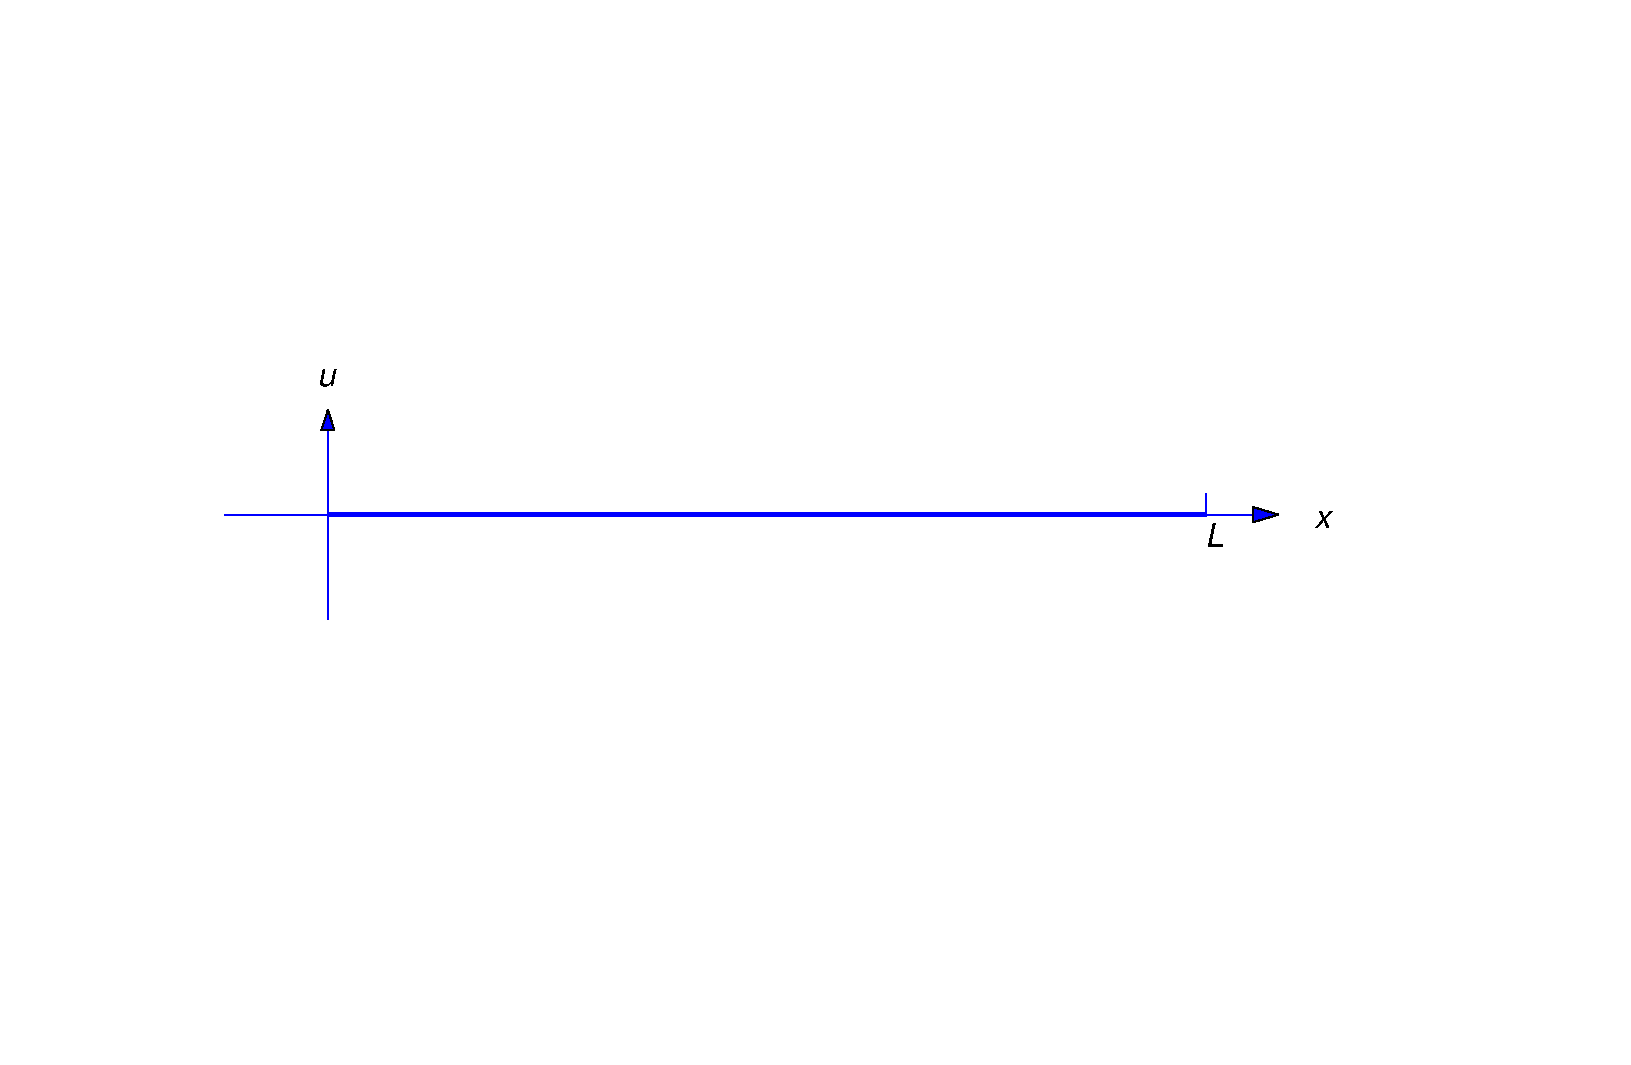
\includegraphics[bb=-78 148 689 643,width=5.67in,height=3.66in,keepaspectratio]{fig120201}
\caption{A stretched string}
  \label{figure:12.2.1}
\end{figure}

If the string is plucked in the vertical direction and released at
time $t=0$, it will oscillate in the $xu$-plane.
Let $u(x,t)$ denote
the displacement of the point on the string above (or below) the
abscissa $x$ at time $t$.

We'll show that it's reasonable to assume that $u$ satisfies the
wave equation under the following assumptions:

\begin{numberlist}
\item % (1)
The mass density (mass per unit length) $\rho$ of the string is
constant throughout the string.
\item % (2)
The tension $T$ induced by tightly stretching the string along the
$x$-axis is so great that all other forces, such as gravity and air
resistance, can be neglected.
\item % (3)
The tension at any point on the
string acts along the tangent to the string at that point,
and the magnitude of its horizontal  component
is always equal to $T$, the tension in the string in equilibrium.
\item % (4)
The slope of the string at every point remains sufficiently small
so that we can make the
approximation
\begin{equation} \label{eq:12.2.2}
\sqrt{1+u_x^2}\approx1.
\end{equation}
\end{numberlist}

Figure~\ref{figure:12.2.2} shows a segment of the displaced string
at a time $t>0$.  (Don't think that the figure  is
necessarily inconsistent
with Assumption~4;     we exaggerated the slope for clarity.)

\begin{figure}[tbp]
  \centering\color{blue}
  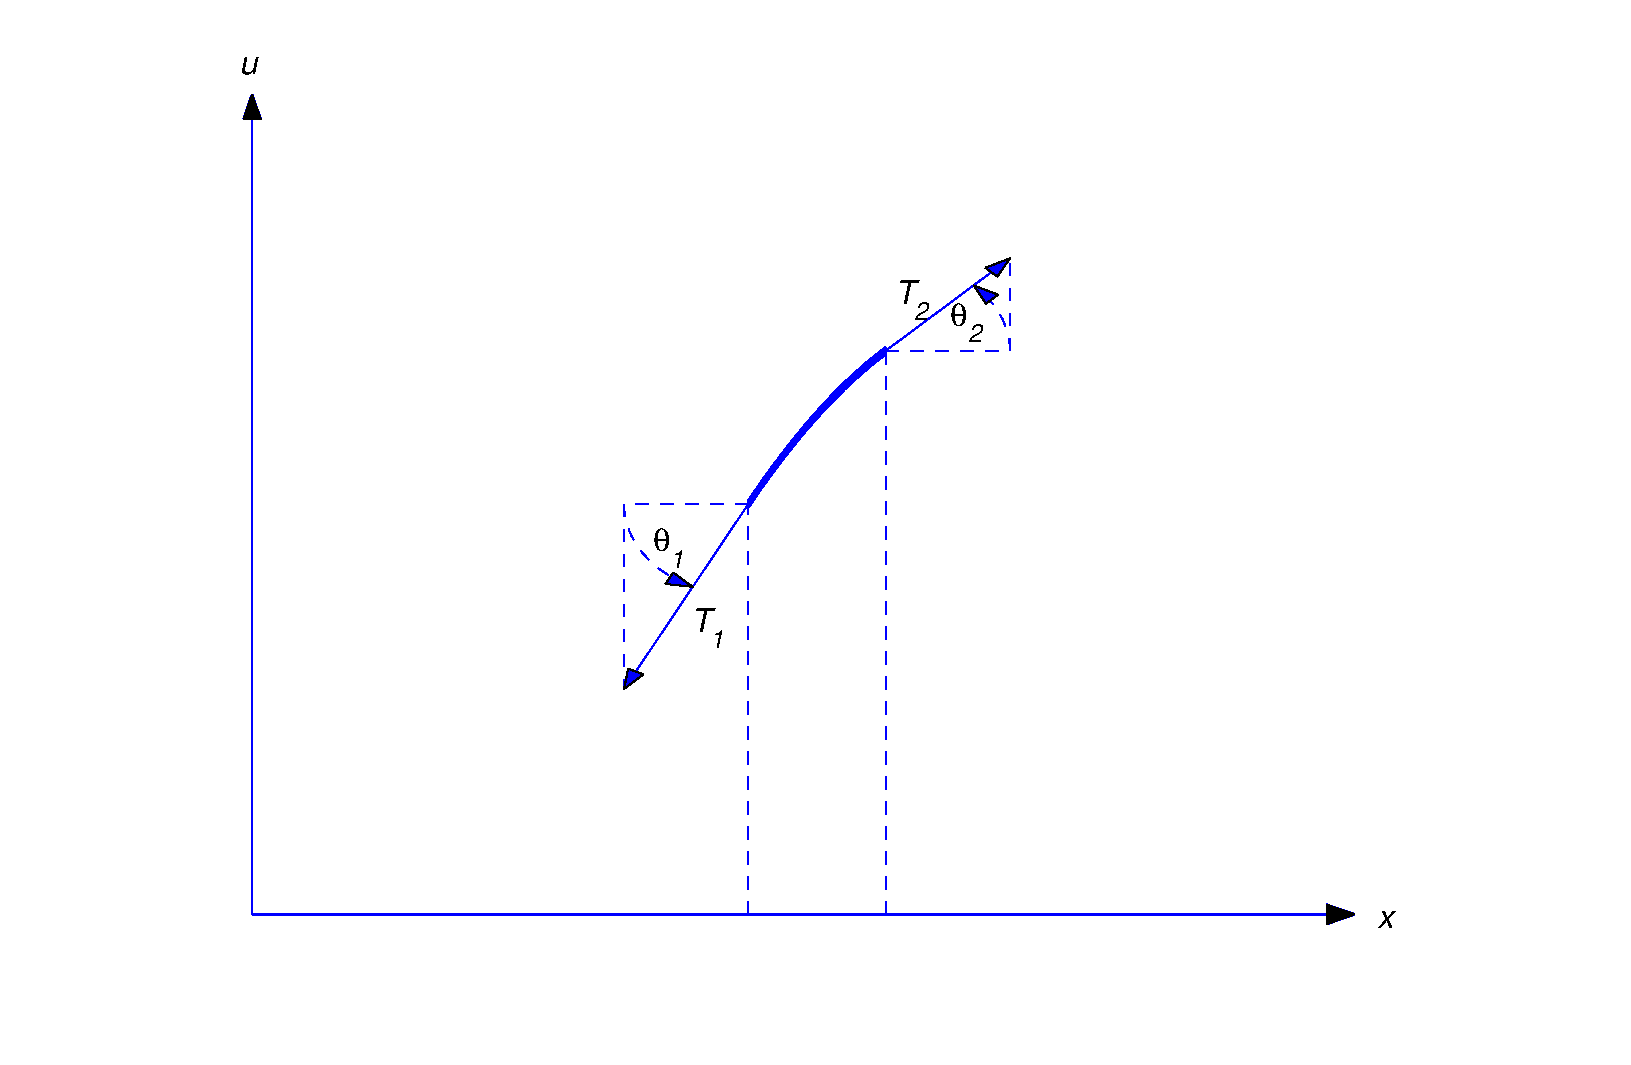
\includegraphics[bb=-78 148 689 643,width=5.67in,height=3.66in,keepaspectratio]{fig120202}
\caption{ A segment of the displaced string}
  \label{figure:12.2.2}
\end{figure}

 The vectors ${\bf T}_1$ and ${\bf T}_2$ are the forces
due to tension, acting along the tangents to the segment at its
endpoints.
From Newton's second law of motion, ${\bf T}_1-{\bf T}_2$
is equal to the mass times the acceleration of the center of
mass of the segment.
The horizontal and vertical components of ${\bf T}_1-{\bf T}_2$
 are
$$
|{\bf T}_2|\cos\theta_2- |{\bf T}_1|\cos\theta_1
\mbox{\quad and \quad}
|{\bf T}_2|\sin\theta_2- |{\bf T}_1|\sin\theta_1,
$$
respectively.
Since
\begin{equation} \label{eq:12.2.3}
|{\bf T}_2|\cos\theta_2=|{\bf T}_1|\cos\theta_1=T
\end{equation}
by assumption, the net horizontal force is zero, so there's
no horizontal acceleration. Since the initial horizontal
velocity is zero, there's no horizontal motion.

Applying Newton's second law of motion in the  vertical direction
yields
\begin{equation} \label{eq:12.2.4}
|{\bf T}_2|\sin\theta_2- |{\bf T}_1|\sin\theta_1=\rho\Delta
s\,u_{tt}(\overline x,t),
\end{equation}
where $\Delta s$ is the length of the segment  and $\overline x$
is the abscissa of the center of mass; hence,
$$
x<\overline x<x+\Delta x.
$$
From calculus, we know that
$$
\Delta s=\int_x^{x+\Delta x}\sqrt{1+u_x^2(\sigma,t)}\,d\sigma;
$$
however, because of \eqref{eq:12.2.2}, we make the approximation
$$
\Delta s\approx\int_x^{x+\Delta x}1\,d\sigma=\Delta x,
$$
so \eqref{eq:12.2.4} becomes
$$
|{\bf T}_2|\sin\theta_2- |{\bf T}_1|\sin\theta_1=\rho\Delta
x\,u_{tt}(\overline x,t).
$$
Therefore
$$
{|{\bf T}_2|\sin\theta_2- |{\bf T}_1|\sin\theta_1\over\Delta x}=\rho
u_{tt}(\overline x,t).
$$
Recalling \eqref{eq:12.2.3}, we divide  by $T$    to obtain
\begin{equation} \label{eq:12.2.5}
{\tan\theta_2-\tan\theta_1\over\Delta x}=
{\rho\over T}u_{tt}(\overline x,t).
\end{equation}
Since
$\tan\theta_1=u_x(x,t)$ and $\tan\theta_2=u_x(x+\Delta x,t)$,
\eqref{eq:12.2.5} is equivalent to
$$
{u_x(x+\Delta x)-u_x(x,t)\over \Delta x}=
{\rho\over T}u_{tt}(\overline x,t).
$$
Letting $\Delta x\to 0$  yields
$$
u_{xx}(x,t)={\rho\over T}u_{tt}(x,t),
$$
which we rewrite as $u_{tt}=a^2u_{xx}$, with $a^2=T/\rho$.

\boxit{The Formal Solution}

\noindent
As in Section~12.1, we use
 separation
of variables to obtain a suitable definition for the formal solution
of \eqref{eq:12.2.1}.
 We begin by looking for functions of the form
$v(x,t)=X(x)T(t)$
that are not identically zero and satisfy
$$
v_{tt}=a^2v_{xx},\quad
v(0,t)=0,\quad v(L,t)=0
$$
for all $(x,t)$.
Since
$$
v_{tt}=XT''\mbox{\quad and \quad}v_{xx}=X''T,
$$
$v_{tt}=a^2v_{xx}$ if and only if
$$
XT''=a^2X''T,
$$
which we rewrite as
$$
{T''\over a^2T}={X''\over X}.
$$
For this  to hold for all $(x,t)$,
 the two sides must equal the same constant;
thus,
$$
{X''\over X}={T''\over a^2T}=-\lambda,
$$
which is equivalent to
$$
X''+\lambda X=0
$$
and
\begin{equation} \label{eq:12.2.6}
T''+a^2\lambda T=0.
\end{equation}
Since $v(0,t)=X(0)T(t)=0$ and $v(L,t)=X(L)T(t)=0$ and we don't want
$T$ to be  identically
zero,  $X(0)=0$ and $X(L)=0$. Therefore $\lambda$
must be an eigenvalue of
\begin{equation} \label{eq:12.2.7}
X''+\lambda X=0,\quad X(0)=0,\quad X(L)=0,
\end{equation}
and $X$ must be a $\lambda$-eigenfunction.
 From Theorem~\ref{thmtype:11.1.2}, the eigenvalues of \eqref{eq:12.2.7}
are $\lambda_n=n^2\pi^2/L^2$, with
associated eigenfunctions
$$
X_n=\sin{n\pi x\over L}, \quad n=1,2,3,\dots.
$$
Substituting $\lambda=n^2\pi^2/L^2$  into
\eqref{eq:12.2.6} yields
$$
T''+(n^2\pi^2a^2/L^2)T=0,
$$
which has the general solution
$$
T_n=\alpha_n\cos{n\pi at\over L}+{\beta_nL\over n\pi a}\sin{n\pi
at\over L},
$$
where $\alpha_n$  and $\beta_n$ are constants. Now let
$$
v_n(x,t)=X_n(x)T_n(t)=\left(\alpha_n\cos{n\pi at\over L}+
{\beta_nL\over n\pi a}\sin{n\pi at\over L}\right)
\sin{n\pi x\over L}.
$$
Then
$$
{\partial v_n\over\partial t}(x,t)=
\left(-{n\pi a \over L}\alpha_n\sin{n\pi at\over L}
+\beta_n\cos{n\pi at\over L}\right)\sin{n\pi x\over L},
$$
so
$$
v_n(x,0)=\alpha_n\sin{n\pi x\over L}
\mbox{\quad and \quad}
{\partial v_n\over\partial t}(x,0)=\beta_n
\sin{n\pi x\over L}.
$$
Therefore $v_n$ satisfies \eqref{eq:12.2.1} with
$f(x)=\alpha_n \sin n\pi x/L$ and  $g(x)=\beta_n\cos n\pi x/L$.
More generally, if $\alpha_1$,  $\alpha_2$, \dots, $\alpha_m$
and $\beta_1$, $\beta_2$,\dots, $\beta_m$ are constants and
$$
u_m(x,t)=\sum_{n=1}^m\left(\alpha_n\cos{n\pi at\over
L}+{\beta_nL\over n\pi a}\sin{n\pi at\over L}\right)
\sin{n\pi x\over L},
$$
then $u_m$ satisfies \eqref{eq:12.2.1} with
$$
f(x)=\sum_{n=1}^m \alpha_n\sin{n\pi x\over L}
\mbox{\quad and \quad}
g(x)=\sum_{n=1}^m \beta_n\sin{n\pi x\over L}.
$$
 This motivates the next definition.

\begin{definition}\color{blue} \label{thmtype:12.2.1}\rm
If $f$ and $g$ are piecewise smooth of $[0,L]$, then
the  formal solution of  \eqref{eq:12.2.1}
is
\begin{equation} \label{eq:12.2.8}
u(x,t)=\sum_{n=1}^\infty\left(\alpha_n\cos{n\pi at\over
L}+{\beta_nL\over n\pi a}\sin{n\pi at\over L}\right)
\sin{n\pi x\over L},
\end{equation}
where
$$
S_f(x)=\sum_{n=1}^\infty \alpha_n\sin{n\pi x\over L}
\mbox{\quad and \quad}
S_{g}(x)=\sum_{n=1}^\infty \beta_n\sin{n\pi x\over L}
$$
are the   Fourier sine series of $f$ and $g$ on $[0,L]$; that is,
$$
\alpha_n={2\over L}\int_0^Lf(x)\sin{n\pi x\over L}\,dx
\mbox{\quad and \quad}
\beta_n={2\over L}\int_0^Lg(x)\sin{n\pi x\over L}\,dx.
$$
\end{definition}

Since there are no  convergence-producing factors in \eqref{eq:12.2.8}
like the negative exponentials in $t$ that appear in formal solutions
of initial-boundary value problems for the heat equation, it isn't
obvious that  \eqref{eq:12.2.8} even converges
for any values of $x$ and $t$, let alone that it can be differentiated
term by term  to show that $u_{tt}=a^2u_{xx}$.
However, the next
theorem guarantees that  the series  converges
not only for $0\le x\le L$  and $t\ge0$, but for $-\infty<x<\infty$
and $-\infty<t<\infty$.

\begin{theorem}\color{blue} \label{thmtype:12.2.2}
If $f$ and $g$ are piecewise smooth on $[0,L]$, then
$u$ in \eqref{eq:12.2.1} converges for all $(x,t)$,
and can be written as
\begin{equation} \label{eq:12.2.9}
u(x,t)={1\over2}[S_f(x+at)+S_f(x-at)]+
{1\over2a}\int_{x-at}^{x+at}S_g(\tau)\,d\tau.
\end{equation}
\end{theorem}

\proof
Setting $A=n\pi x/L$ and $B=n\pi at/L$ in the  identities
$$
\sin A\cos B=\phantom{-}{1\over2}[\sin(A+B)+\sin(A-B)]
$$
and
$$
\sin A\sin B=-{1\over2}[\cos(A+B)-\cos(A-B)]
$$
yields
\begin{equation} \label{eq:12.2.10}
\cos{n\pi at\over L}\sin{n\pi x\over L}
={1\over2}\left[\sin{n\pi(x+at)\over
L}+\sin{n\pi(x-at)\over L}\right]
\end{equation}
and
\begin{equation} \label{eq:12.2.11}
\begin{array}{rcl}
\dst \sin{n\pi at\over L}\sin{n\pi x\over L}
&=&-\dst{1\over2}\left[\cos{n\pi(x+at)\over
L}-\cos{n\pi(x-at)\over
L}\right]\\&=&\dst{n\pi\over2L}\int_{x-at}^{x+at}
\sin{n\pi\tau\over L}\,d\tau.
\end{array}
\end{equation}
From  \eqref{eq:12.2.10},
\begin{equation} \label{eq:12.2.12}
\begin{array}{rcl}
\dst\sum_{n=1}^\infty\alpha_n \cos{n\pi at\over L}\sin{n\pi x\over
L}&=&
\dst{1\over2}\sum_{n=1}^\infty\alpha_n\left(\sin{n\pi(x+at)\over
L}
+\sin{n\pi(x-at)\over L}\right)\\
&=&\dst{1\over2}[S_f(x+at)+S_f(x-at)].
\end{array}
\end{equation}
Since it can be shown that a Fourier sine series can be integrated
term by term between any two limits,
\eqref{eq:12.2.11} implies that
$$
\begin{array}{rcl}
\dst\sum_{n=1}^\infty{\beta_nL\over n\pi a}
\sin{n\pi at\over L}\sin{n\pi x\over L}&=&
\dst{1\over2a}\sum_{n=1}^\infty \beta_n\int_{x-at}^{x+at}
\sin{n\pi\tau\over L}\,d\tau\\
&=&\dst{1\over2a}\int_{x-at}^{x+at}\left(\sum_{n=1}^\infty \beta_n
\sin{n\pi\tau\over L}\right)\,d\tau\\
&=&
\dst{1\over2a}\int_{x-at}^{x+at}S_g(\tau)\,d\tau.
\end{array}
$$
This and  \eqref{eq:12.2.12} imply \eqref{eq:12.2.9},
which completes the proof.

As we'll see below, if $S_g$ is differentiable and $S_f$
is twice differentiable on $(-\infty,\infty)$, then
\eqref{eq:12.2.9} satisfies $u_{tt}=a^2u_{xx}$ for all $(x,t)$. We need the
next theorem to formulate conditions on $f$ and $g$ such that
$S_f$ and $S_g$ to have these properties.

\begin{theorem}\color{blue} \label{thmtype:12.2.3}
Suppose $h$ is differentiable on $[0,L]$; that is,
$h'(x)$ exists for $0<x<L$, and the one-sided derivatives
$$
h'_+(0)=\lim_{x\to0+}{h(x)-h(0)\over x}
\mbox{\quad and \quad}
h'_-(L)=\lim_{x\to L-}{h(x)-h(L)\over x-L}
$$
both exist.

\part{a}
Let $p$ be the odd periodic extension of $h$ to $(-\infty,\infty)$;
that is,
$$
p(x)=
\left\{\begin{array}{cl}
h(x),&\quad 0\le x\le L,\\
-h(-x),&-L<x<0,
\end{array}\right.
\mbox{\  and\  } p(x+2L)=p(x),\quad -\infty<x<\infty.
$$
Then $p$ is differentiable on $(-\infty,\infty)$ if and only
if
\begin{equation} \label{eq:12.2.13}
h(0)=h(L)=0.
\end{equation}

\part{b}
Let $q$ be the even periodic extension of $h$ to $(-\infty,\infty)$;
that is,
$$
q(x)=
\left\{\begin{array}{cl}
h(x),&\quad 0\le x\le L,\\
h(-x),&-L<x<0,
\end{array}\right.
\mbox{\  and\  } q(x+2L)=q(x),\quad -\infty<x<\infty.
$$
Then $q$ is differentiable on $(-\infty,\infty)$ if and only
if
\begin{equation} \label{eq:12.2.14}
h'_+(0)=h'_-(L)=0.
\end{equation}
\end{theorem}

\proof
Throughout this proof, $k$ denotes an integer.
Since $f$ is differentiable on the open interval
$(0,L)$, both $p$ and $q$ are differentiable on every
open interval $((k-1)L,kL)$. Thus, we need
only to  determine whether $p$ and $q$ are differentiable
at $x=kL$ for every  $k$.

\part{a}
From Figure~\ref{figure:12.2.3},
 $p$ is discontinuous at $x=2kL$ if $h(0)\ne0$
and   discontinuous at $x=(2k-1)L$ if $h(L)\ne0$.
Therefore $p$
is not differentiable on $(-\infty,\infty)$  unless $h(0)=h(L)=0$.
From
 Figure~\ref{figure:12.2.4}, if $h(0)=h(L)=0$, then
$$
p'(2kL)=h_+'(0)\mbox{\quad and \quad}p'((2k-1)L)=h_-'(L)
$$
for every  $k$;  therefore, $p$ is differentiable on
$(-\infty,\infty)$.

\begin{figure}[htbp]
\color{blue}
  \begin{minipage}[b]{0.5\linewidth}
    \centering
   \scalebox{.55}{
  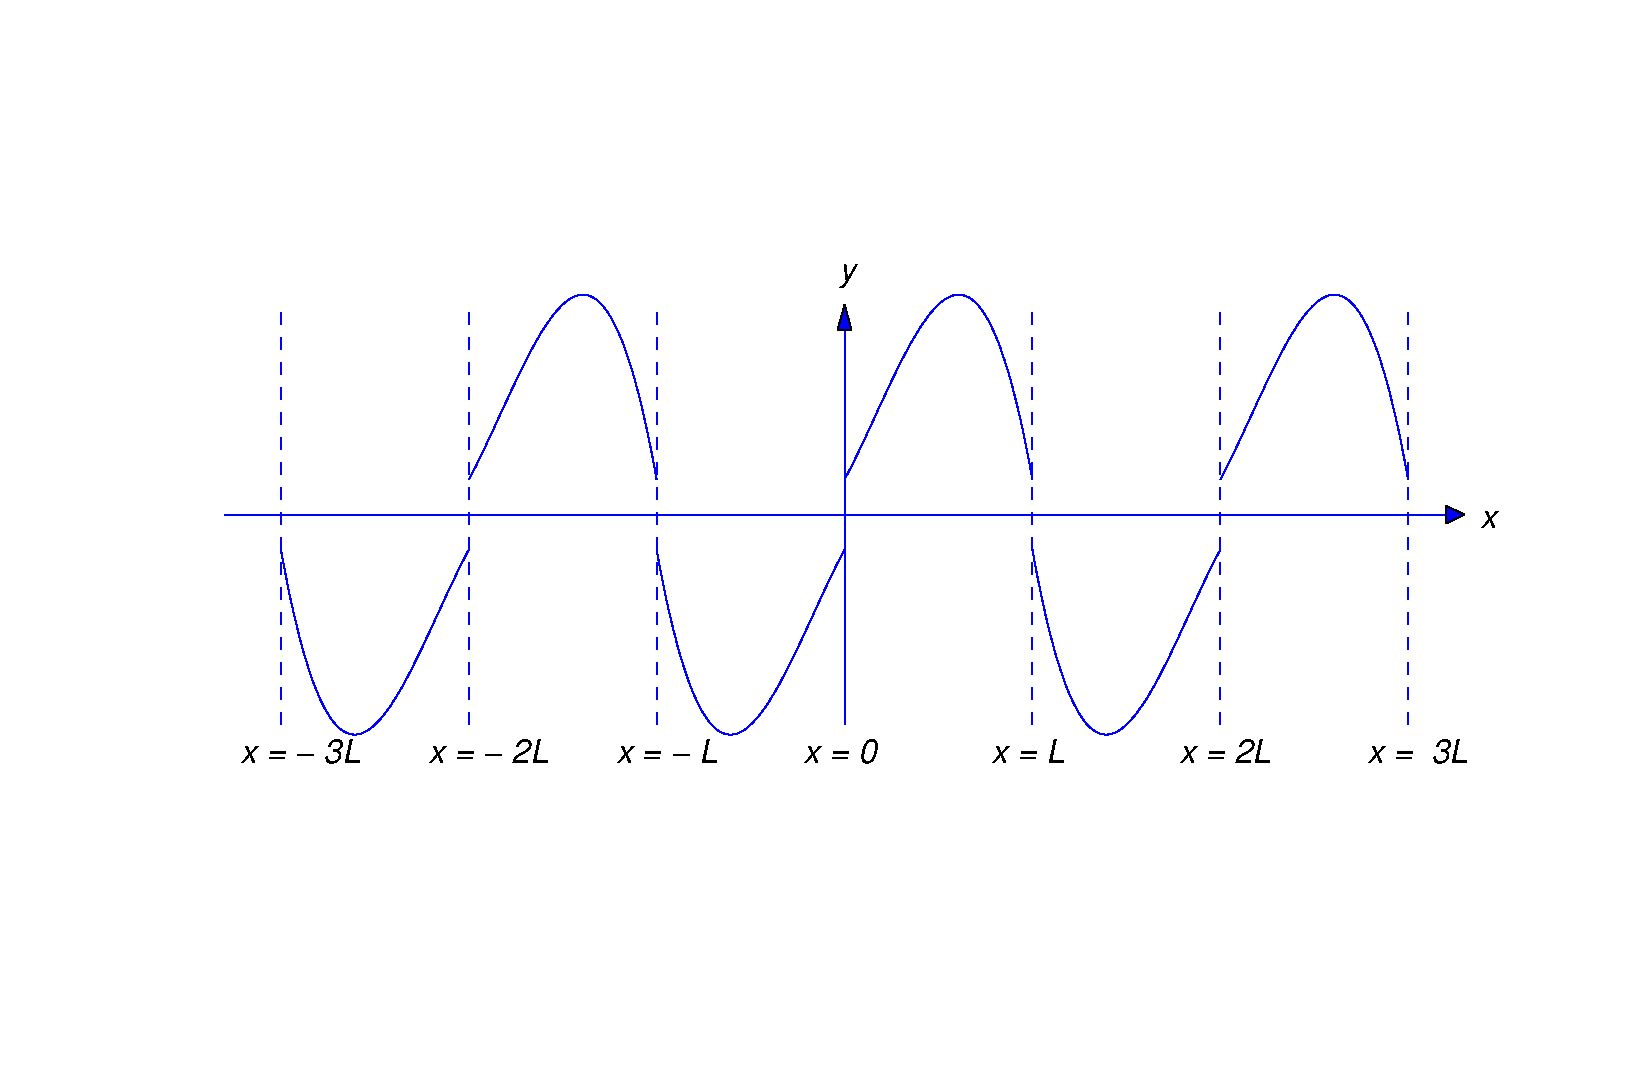
\includegraphics[bb=-78 148 689 643,width=5.67in,height=3.66in,keepaspectratio]{fig120203}}
\caption{ The odd extension of a function that does
not satisfy \eqref{eq:12.2.13}}
  \label{figure:12.2.3}
\end{minipage}
  \begin{minipage}[b]{0.5\linewidth}
    \centering
   \scalebox{.55}{
  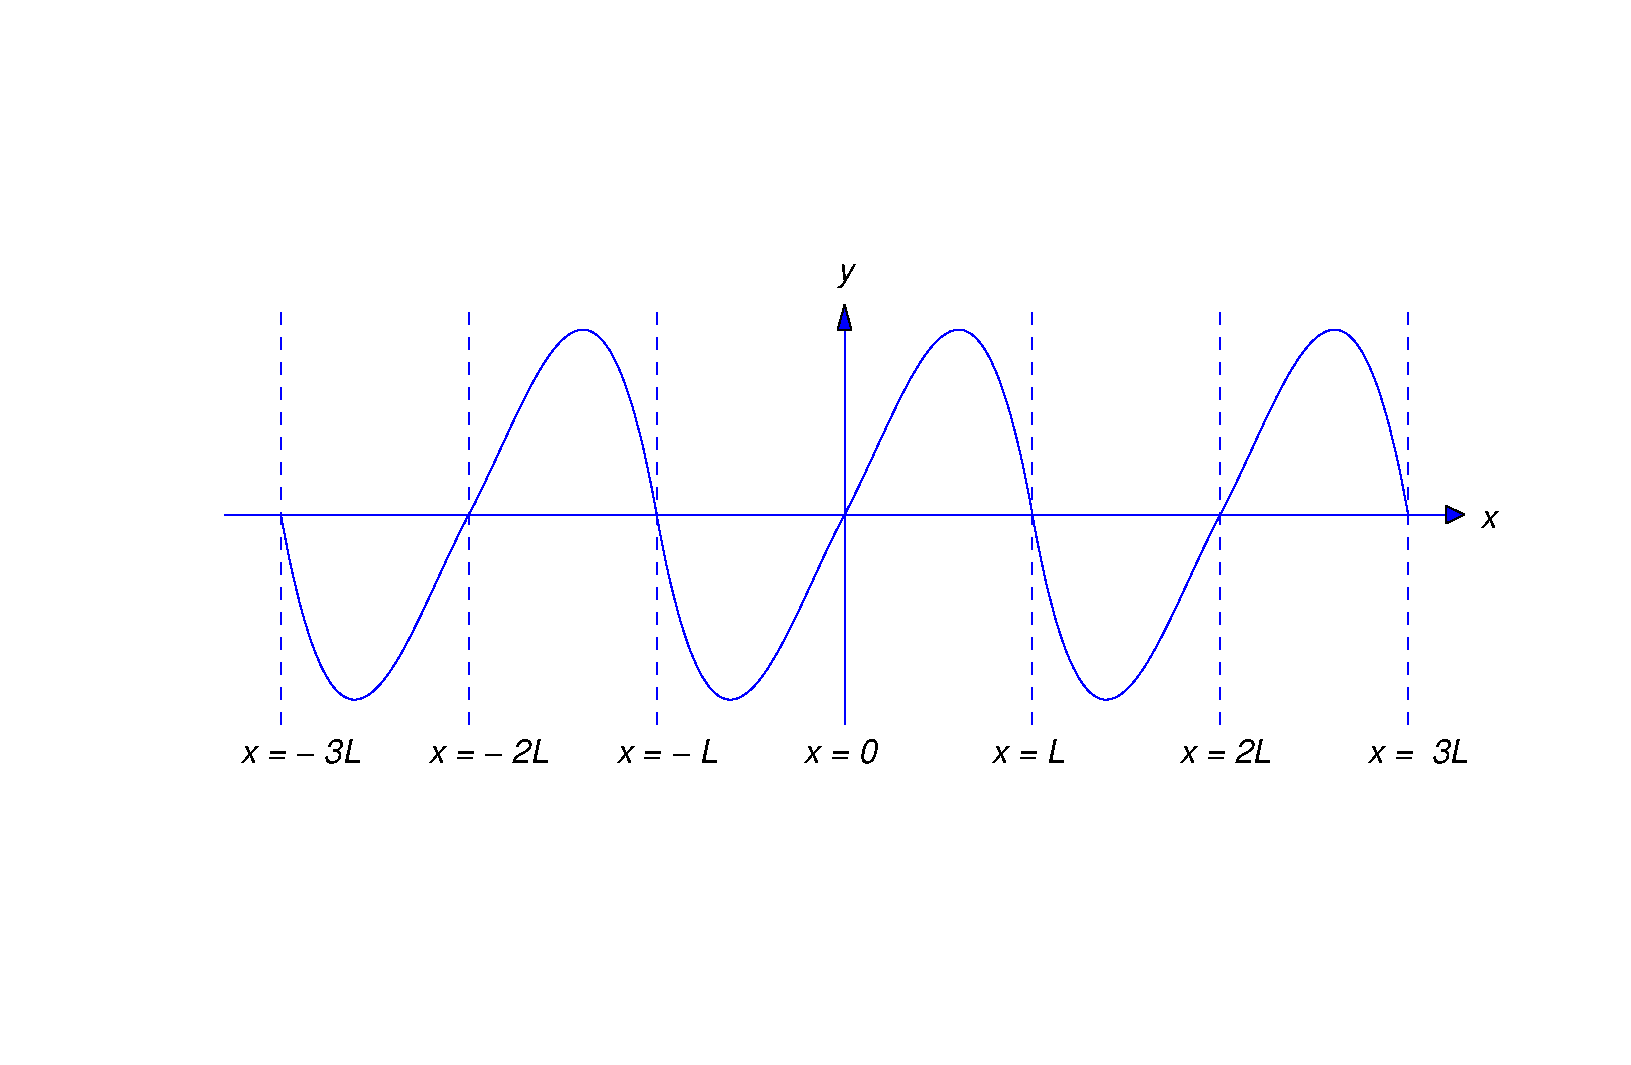
\includegraphics[bb=-78 148 689 643,width=5.67in,height=3.66in,keepaspectratio]{fig120204}}
\caption{ The odd extension of a function that
 satisfies \eqref{eq:12.2.13}}
  \label{figure:12.2.4}
\end{minipage}
\end{figure}

\part{b}
From Figure~\ref{figure:12.2.5},
$$
q'_-(2kL)=-h'_+(0)\mbox{\quad and \quad}  q'_+(2kL)=h'_+(0),
$$
so $q$ is differentiable at $x=2kL$ if and only if $h'_+(0)=0$.
Also,
$$
q'_-((2k-1)L)=h'_-(L) \mbox{\quad and \quad} q'_+((2k-1)L)=-h'_-(L),
$$
so $q$ is differentiable at $x=(2k-1)L$ if and only if $h'_-(L)=0$.
Therefore
 $q$  is differentiable on $(-\infty,\infty)$
if and only if $h'_+(0)=h'_-(L)=0$, as in Figure~\ref{figure:12.2.6}.
This completes the proof.

\begin{figure}[H]
\color{blue}
  \begin{minipage}[b]{0.5\linewidth}
    \centering
   \scalebox{.55}{
  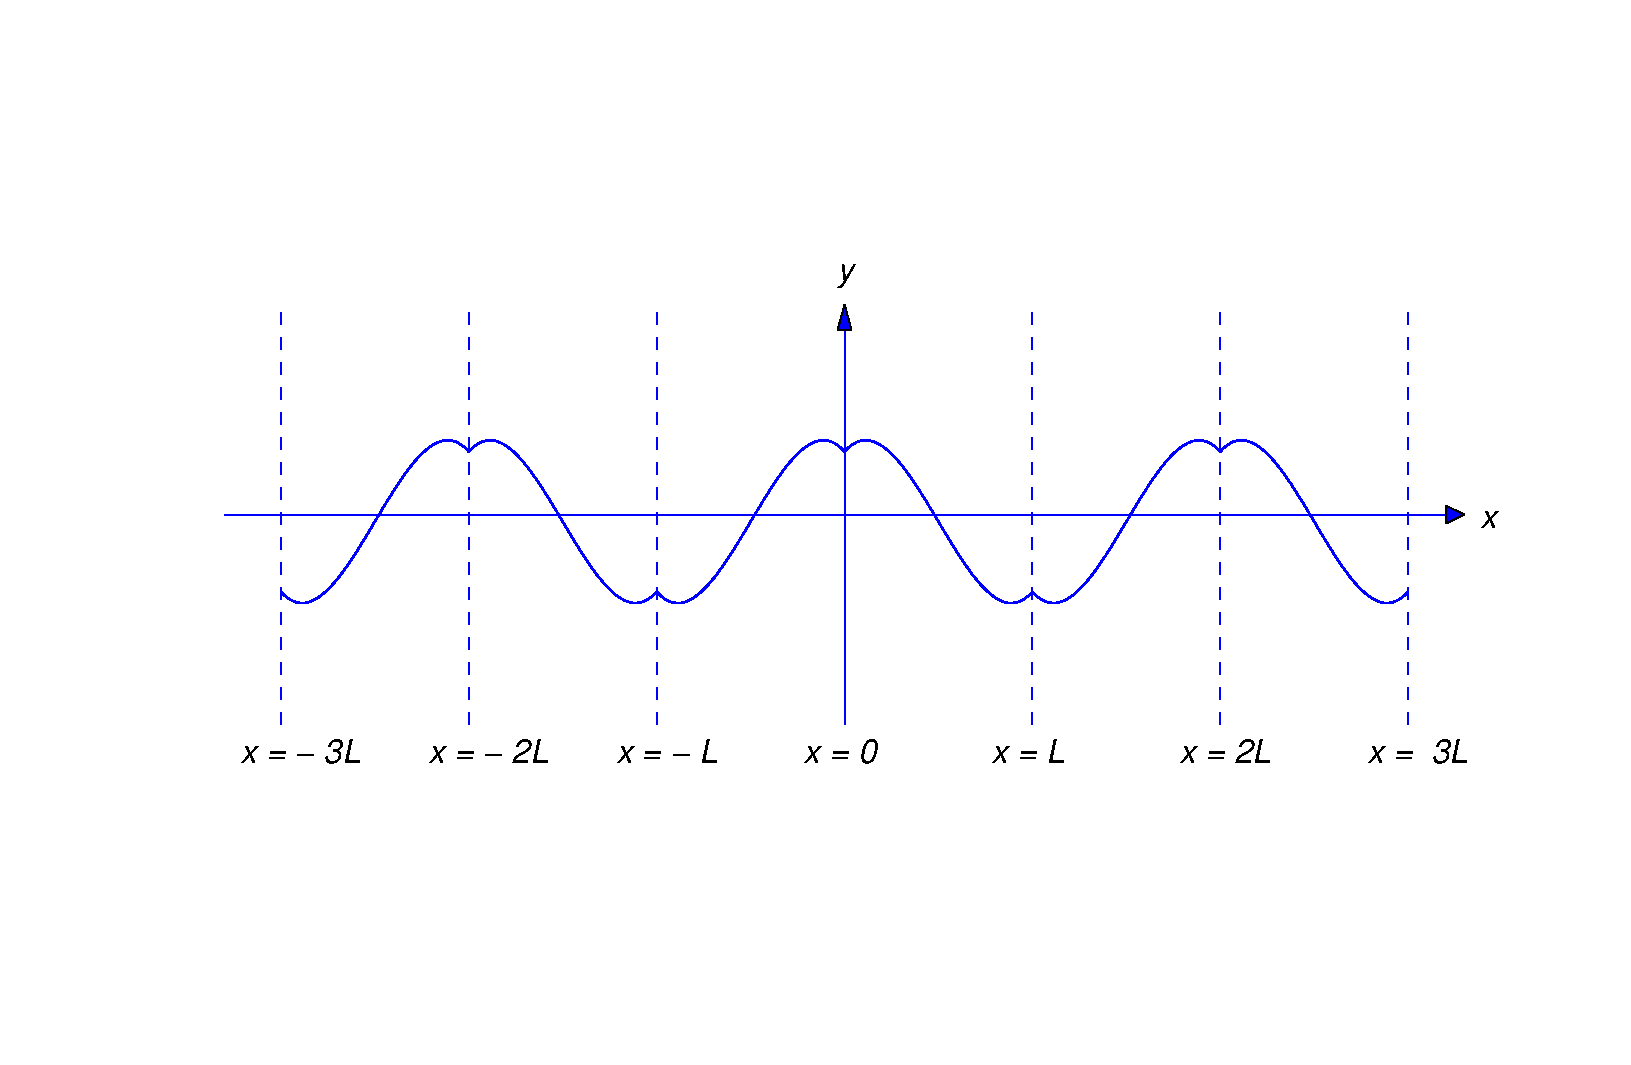
\includegraphics[bb=-78 148 689 643,width=5.67in,height=3.66in,keepaspectratio]{fig120205}}
\caption{ The even extension of a function that doesn't
 satisfy \eqref{eq:12.2.14}}
  \label{figure:12.2.5}
\end{minipage}
  \begin{minipage}[b]{0.5\linewidth}
    \centering
   \scalebox{.55}{
  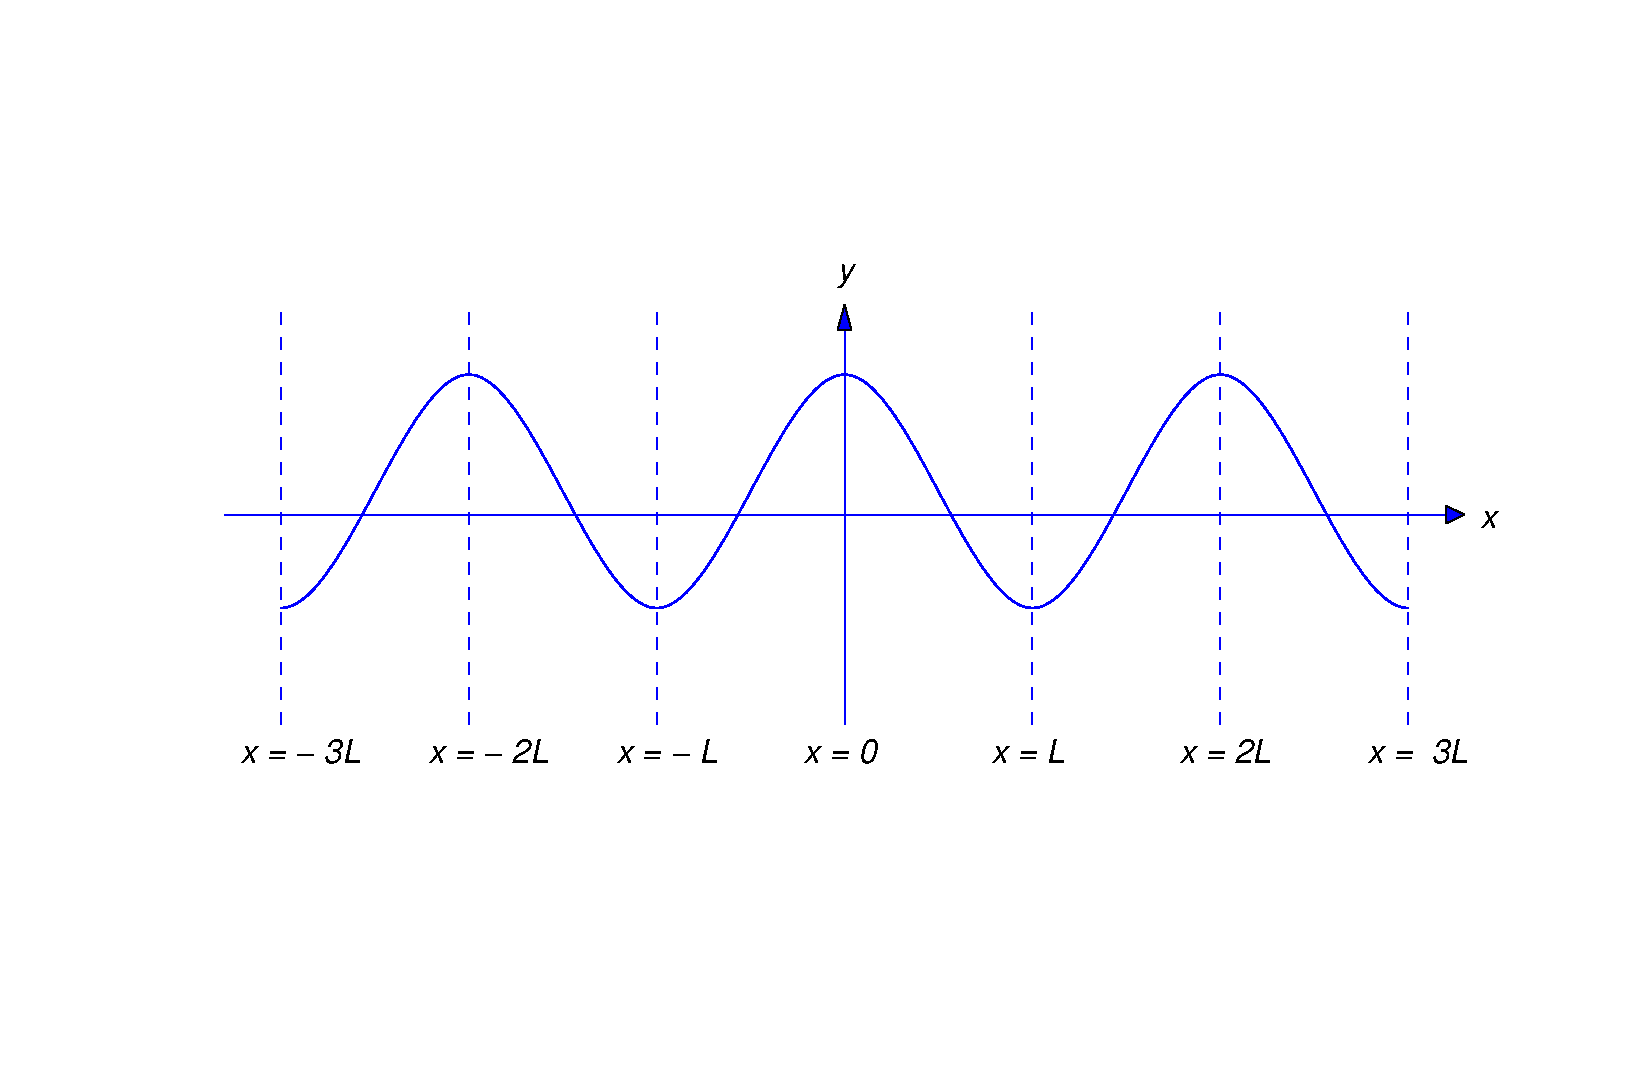
\includegraphics[bb=-78 148 689 643,width=5.67in,height=3.66in,keepaspectratio]{fig120206}}
\caption{ The even extension of a function that
 satisfies \eqref{eq:12.2.14}}
  \label{figure:12.2.6}
\end{minipage}
\end{figure}

\begin{theorem}\color{blue} \label{thmtype:12.2.4}
The formal solution of \eqref{eq:12.2.1}
is an actual solution if $g$ is differentiable on $[0,L]$
and
\begin{equation} \label{eq:12.2.15}
g(0)=g(L)=0,
\end{equation}
while $f$ is twice differentiable on $[0,L]$ and
\begin{equation} \label{eq:12.2.16}
f(0)=f(L)=0
\end{equation}
and
\begin{equation} \label{eq:12.2.17}
f''_+(0)=f''_-(L)=0.
\end{equation}
\end{theorem}

\proof
We first show that $S_g$ is differentiable and $S_f$
is twice differentiable on $(-\infty,\infty)$. We'll then
differentiate  \eqref{eq:12.2.9} twice with respect to $x$ and $t$
and verify that  \eqref{eq:12.2.9}  is an actual solution of \eqref{eq:12.2.1}.

Since  $f$ and $g$ are continuous on $(0,L)$,
 Theorem~\ref{thmtype:11.3.2} implies that
$S_f(x)=f(x)$ and $S_g(x)=g(x)$ on $[0,L]$. Therefore $S_f$
and $S_g$ are the odd periodic extensions  of $f$ and $g$.
 Since $f$ and $g$ are differentiable on $[0,L]$,
\eqref{eq:12.2.15},
\eqref{eq:12.2.16}, and  Theorem~\ref{thmtype:12.2.3}\part{a} imply that
$S_f$ and $S_g$ are differentiable on $(-\infty,\infty)$.

Since $S_f'(x)=f'(x)$ on $[0,L]$ (one-sided derivatives at the
endpoints), and
$S_f'$ is even
(the derivative of an odd function is even),
$S_f'$ is the even periodic extension of $f'$. By assumption, $f'$ is
differentiable on $[0,L]$. Because of \eqref{eq:12.2.17},
Theorem~\ref{thmtype:12.2.3}\part{b} with $h=f'$ and $q=S_f'$ implies that
$S_f''$ exists on $(-\infty,\infty)$.

Now we can differentiate \eqref{eq:12.2.9} twice with respect to $x$
and $t$:
$$
u_x(x,t)={1\over2}[S_f'(x+at)+S_f'(x-at)]+
{1\over2a}[S_g(x+at)-S_g(x-at)],
$$
\begin{equation} \label{eq:12.2.18}
u_{xx}(x,t)={1\over2}[S_f''(x+at)+S_f''(x-at)]+
{1\over2a}[S_g'(x+at)-S_g'(x-at)],
\end{equation}
\begin{equation} \label{eq:12.2.19}
u_t(x,t)={a\over2}[S_f'(x+at)-S_f'(x-at)]+
{1\over2}[S_g(x+at)+S_g(x-at)],
\end{equation}
and
\begin{equation} \label{eq:12.2.20}
u_{tt}(x,t)={a^2\over2}[S_f''(x+at)-S_f''(x-at)]+
{a\over2}[S_g'(x+at)-S_g'(x-at)].
\end{equation}
Comparing \eqref{eq:12.2.18}  and \eqref{eq:12.2.20} shows that
$u_{tt}(x,t)=a^2u_{xx}(x,t)$ for all $(x,t)$.

From \eqref{eq:12.2.8},  $u(0,t)=u(L,t)=0$
for all $t$. From \eqref{eq:12.2.9},
$u(x,0)=S_f(x)$ for all $x$, and therefore, in particular,
$$
u(x,0)=f(x),\quad 0\le x< L.
$$
 From \eqref{eq:12.2.19},
$u_t(x,0)=S_g(x)$ for all $x$, and therefore, in particular,
$$
u_t(x,0)=g(x),\quad 0\le x< L.
$$
Therefore $u$ is an actual solution of \eqref{eq:12.2.1}.
This completes the proof.

Eqn~\eqref{eq:12.2.9} is called
\href{https://mathshistory.st-andrews.ac.uk/Biographies/DAlembert/}
{\color{blue}\it d'Alembert's
 solution\/} of \eqref{eq:12.2.1}. Although
d'Alembert's solution   was useful
for proving Theorem~\ref{thmtype:12.2.4} and is very useful in a slightly
different context (Exercises~\ref{exer:12.2.63}-\ref{exer:12.2.68}),
\eqref{eq:12.2.8} is preferable for computational purposes.

\begin{example}\label{example:12.2.1} \rm
Solve \eqref{eq:12.2.1} with
$$
f(x)=x(x^3-2Lx^2+L^2)
\mbox{\quad and \quad}
g(x)=x(L-x).
$$
\end{example}

\solution
We leave it to you to verify that $f$ and $g$ satisfy the assumptions
of Theorem~\ref{thmtype:12.2.4}.

From Exercise~11.3.~\hspace*{-3pt}\ref{exer:11.3.39},
$$
S_f(x)={96L^4\over\pi^5}\sum_{n=1}^\infty{1\over(2n-1)^5}\sin{(2n-1)\pi
x\over L}.
$$
From Exercise~11.3.~\hspace*{-3pt}\ref{exer:11.3.36},
$$
S_g(x)={8L^2\over\pi^3}\sum_{n=1}^\infty{1\over(2n-1)^3}\sin{(2n-1)\pi
x\over L}.
$$
From \eqref{eq:12.2.8},
$$
\begin{array}{rcl}
u(x,t)&=&
\dst{96L^4\over\pi^5}\sum_{n=1}^\infty{1\over(2n-1)^5}
\cos{(2n-1)\pi a t\over L}\sin{(2n-1)\pi x\over L}\\&&+
\dst{8L^3\over a\pi^4}\sum_{n=1}^\infty{1\over(2n-1)^4}
\sin{(2n-1)\pi a t\over L}\sin{(2n-1)\pi x\over L}.
\end{array}
$$

Theorem~\ref{thmtype:12.1.2}  implies that $u_{xx}$
and $u_{tt}$    can be obtained by term
by term differentiation, for all
$(x,t)$, so $u_{tt}=a^2u_{xx}$ for all
$(x,t)$ (Exercise~\ref{exer:12.2.62}). Moreover,
Theorem~\ref{thmtype:11.3.2}
implies that $S_f(x)=f(x)$ and $S_g(x)=g(x)$ if $0\le x\le L$. Therefore
$u(x,0)=f(x)$ and $u_t(x,0)=g(x)$ if $0\le x\le L$.
Hence, $u$ is an actual solution of the initial-boundary
value problem.

\medskip

\color{blue}
\remark
{In solving a specific initial-boundary value problem \eqref{eq:12.2.1},
it's convenient to solve the problem with $g\equiv0$, then with
$f\equiv0$, and add the solutions to obtain the solution of the given
problem. Because of this, either $f\equiv0$ or $g\equiv0$ in all
the specific initial-boundary value problems in the exercises.}
\color{black}

\boxit{The Plucked String}

\noindent
If $f$ and $g$ don't satisfy the assumptions of
Theorem~\ref{thmtype:12.2.4}, then \eqref{eq:12.2.8} isn't  an actual
solution of \eqref{eq:12.2.1}   in fact, it can be shown that \eqref{eq:12.2.1}
doesn't have an
actual solution in this case. Nevertheless, $u$ is defined for all
$(x,t)$, and we can see from \eqref{eq:12.2.18} and \eqref{eq:12.2.20} that
$u_{tt}(x,t)=a^2u_{xx}(x,t)$ for all $(x,t)$ such that
$S_f''(x\pm at)$  and $S_g'(x\pm at)$ exist.  Moreover, $u$
may still provide a useful approximation to the vibration of the
string;    a laboratory experiment can confirm or deny this.

We'll now consider the initial-boundary value problem
 \eqref{eq:12.2.1}  with
\begin{equation} \label{eq:12.2.21}
f(x)=
\left\{\begin{array}{cl}
x,&0\le x\le{L\over2},\\L-x,&{L\over2}\le x\le L
\end{array}\right.
\end{equation}
and $g\equiv0$.
Since $f$ isn't  differentiable at $x=L/2$, it doesn't satisfy
the assumptions of Theorem~\ref{thmtype:12.2.4}, so the formal solution
of \eqref{eq:12.2.1} can't be an actual solution.
Nevertheless,
it's instructive to investigate the properties of the formal
solution.

The graph of $f$ is shown in Figure~\ref{figure:12.2.7}. Intuitively, we
are plucking the string by half its length at the middle. You're right
if you think this is an extraordinarily large displacement;
however, we could remove this objection by multiplying the function in
Figure~\ref{figure:12.2.7} by a small constant. Since this would just
multiply the formal solution by the same constant, we'll leave $f$ as
we've defined it. Similar comments apply to the exercises.

\begin{figure}[tbp]
  \centering\color{blue}
  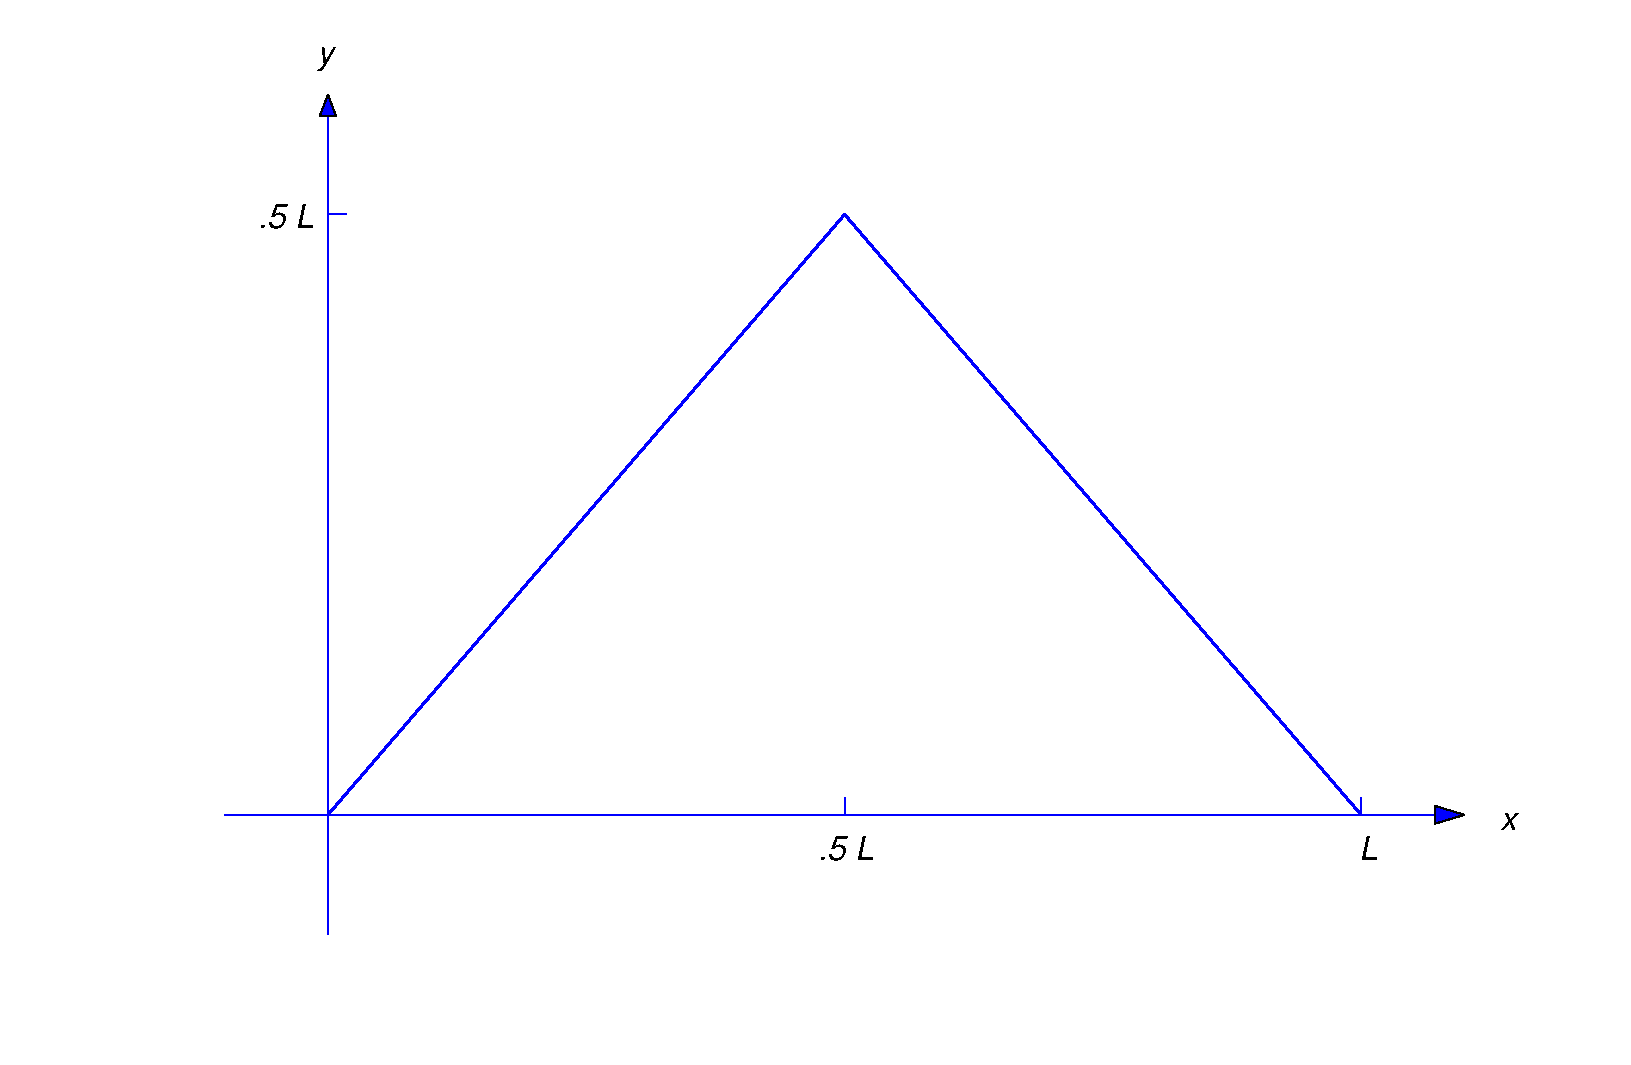
\includegraphics[bb=-78 148 689 643,width=5.67in,height=3.66in,keepaspectratio]{fig120207}
\caption{Graph of \eqref{eq:12.2.21}}
  \label{figure:12.2.7}
\end{figure}

From Exercise~11.3.~\hspace*{-3pt}\ref{exer:11.3.15}, the Fourier sine
series
of
$f$ on $[0,L]$ is
$$
S_f(x)=\dst{4L\over\pi^2}\sum_{n=1}^\infty{(-1)^{n+1}\over(2n-1)^2}
\sin{(2n-1)\pi x\over L},
$$
which converges to $f$ for all $x$ in $[0,L]$, by
Theorem~\ref{thmtype:11.3.2}. Therefore
\begin{equation} \label{eq:12.2.22}
u(x,t)=\dst{4L\over\pi^2}\sum_{n=1}^\infty{(-1)^{n+1}\over(2n-1)^2}
\cos{(2n-1)\pi at\over L}\sin{(2n-1)\pi x\over L}.
\end{equation}
This series converges absolutely for all $(x,t)$ by the comparison
test, since the series
$$
\sum_{n=1}^\infty{1\over(2n-1)^2}
$$
 converges. Moreover, \eqref{eq:12.2.22} satisfies the boundary
conditions
$$
u(0,t)=u(L,t)=0,\quad t>0,
$$
and the initial condition
$$
u(x,0)=f(x),\quad  0\le x\le L.
$$
However, we can't justify differentiating \eqref{eq:12.2.22} term by
term even once, and formally differentiating  it twice
term by term produces a series that diverges for all $(x,t)$.
(Verify.). Therefore
 we use
 d'Alembert's form
\begin{equation} \label{eq:12.2.23}
u(x,t)={1\over2}[S_f(x+at)+S_f(x-at)]
\end{equation}
for $u$ to study its derivatives.
Figure~\ref{figure:12.2.8} shows the graph of $S_f$, which is  the
odd periodic extension of $f$. You can see  from the graph
that $S_f$ is differentiable at  $x$ (and $S_f'(x)=\pm1$) if
and only if
$x$ isn't  an odd multiple of
$L/2$.

\begin{figure}[H]
\color{blue}
  \begin{minipage}[b]{0.5\linewidth}
    \centering
   \scalebox{.65}{
  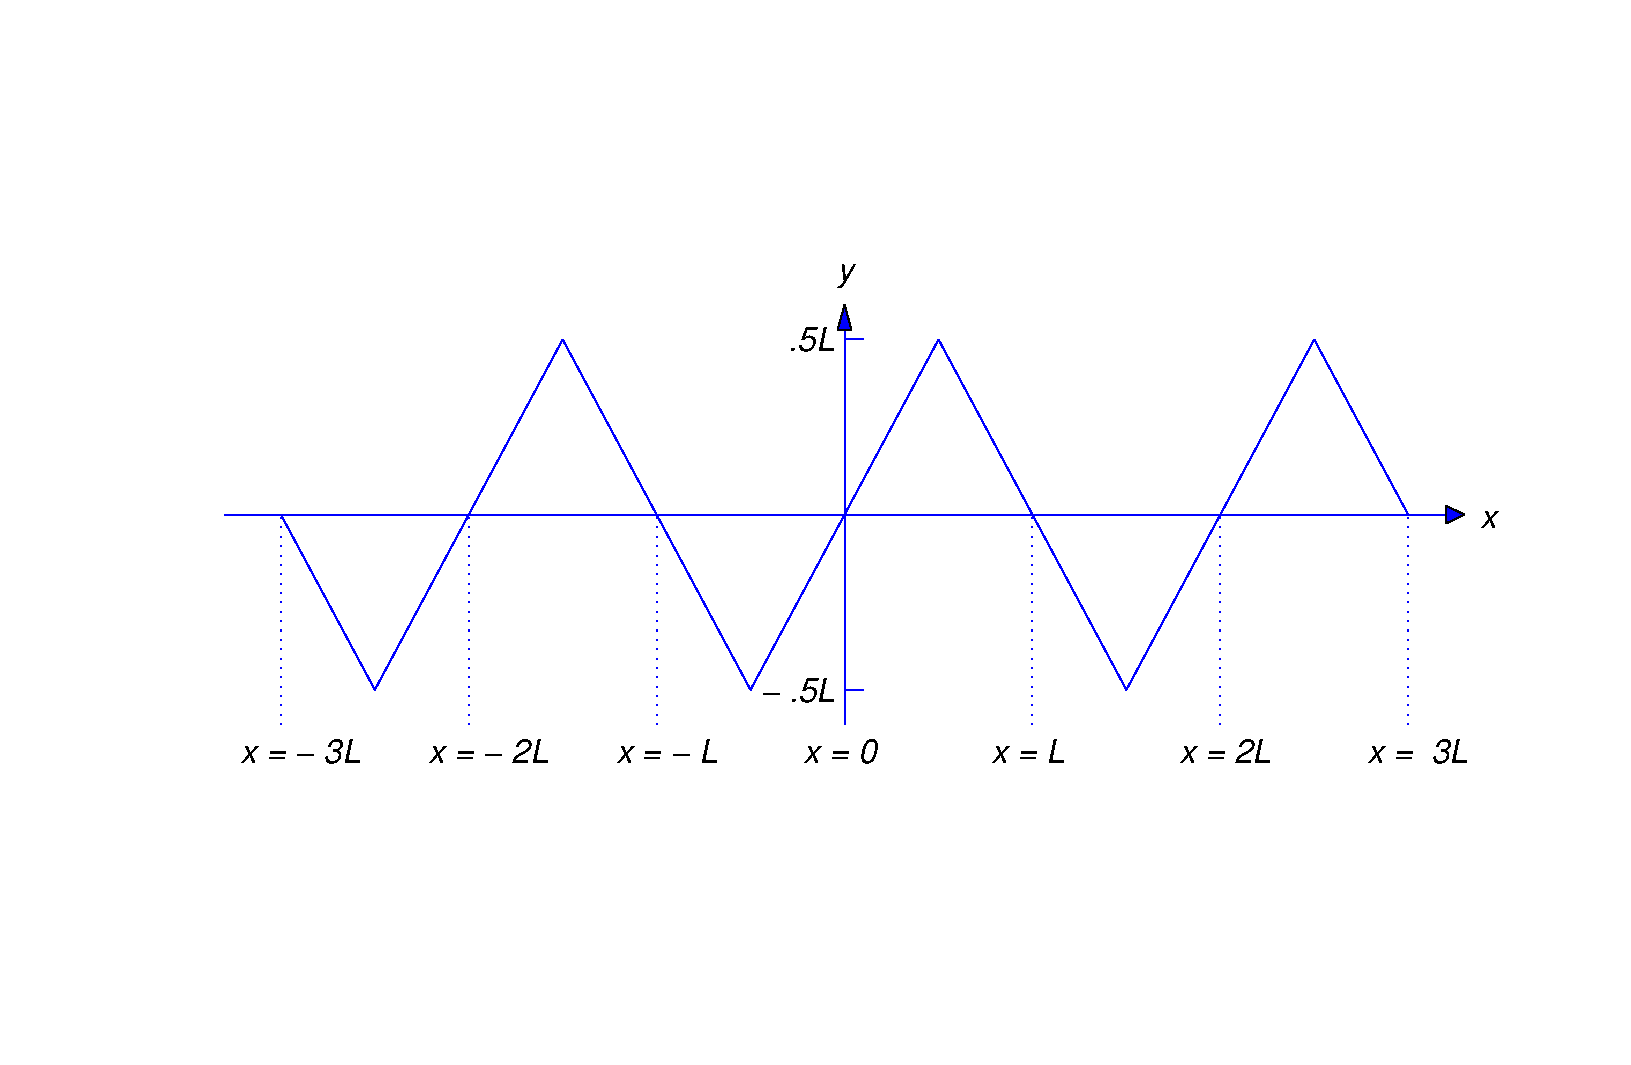
\includegraphics[bb=-78 148 689 643,width=5.67in,height=3.66in,keepaspectratio]{fig120208}}
\caption{ The odd periodic extension of
\eqref{eq:12.2.21}}
  \label{figure:12.2.8}
\end{minipage}
  \begin{minipage}[b]{0.5\linewidth}
    \centering
   \scalebox{.65}{
  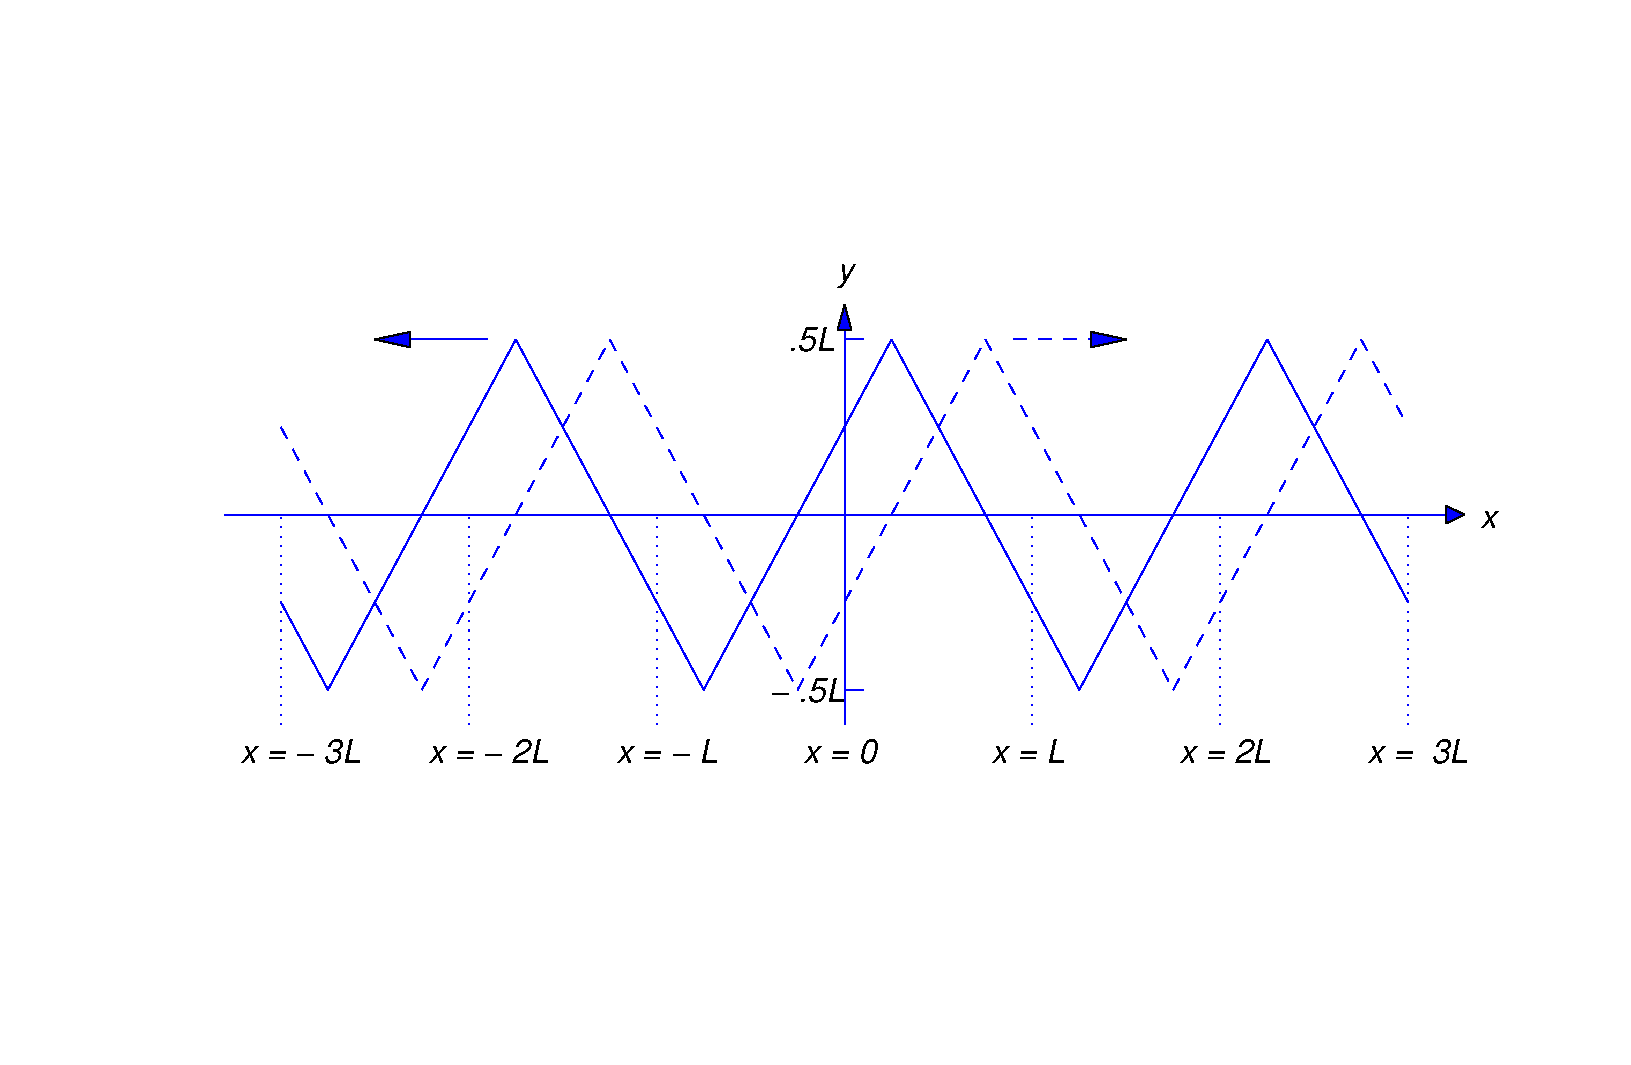
\includegraphics[bb=-78 148 689 643,width=5.67in,height=3.66in,keepaspectratio]{fig120209}}
\caption{ Graphs of $y=S_f(x-at)$ (dashed) and $y=S_f(x-at)$ (solid),
with $f$ as in \eqref{eq:12.2.21}}
  \label{figure:12.2.9}
\end{minipage}
\end{figure}

In Figure~\ref{figure:12.2.9} the
dashed and solid curves  are the graphs of $y=S_f(x-at)$ and
$y=S_f(x+at)$ respectively, for a fixed value of $t$.
As $t$ increases the dashed curve moves to the right and the solid
curve moves to the left. For this reason, we say that the functions
$u_1(x,t)=S_f(x+at)$ and $u_2(x,t)=S_f(x-at)$ are {\color{blue}\it traveling
waves\/}.
Note that $u_1$ satisfies the wave equation at $(x,t)$
if $x+at$ isn't  an odd multiple of $L/2$ and
 $u_2$ satisfies the wave equation at  $(x,t)$ if
$x-at$ isn't  an odd  multiple of $L/2$. Therefore \eqref{eq:12.2.23}
(or, equivalently, \eqref{eq:12.2.22})  satisfies
$u_{tt}(x,t)=a^2u_{xx}(x,t)=0$ for all $(x,t)$ such that neither
$x-at$ nor $x+at$ is an odd multiple of $L/2$.

We conclude by finding an  explicit formula for $u(x,t)$
 under the assumption that
\begin{equation} \label{eq:12.2.24}
0\le x\le L\mbox{\quad and \quad}0\le t\le L/2a.
\end{equation}
To see how this formula can be used to compute $u(x,t)$ for
$0\le x\le L$ and arbitrary
$t$, we refer you to Exercise~\ref{exer:12.2.16}.

From Figure~\ref{figure:12.2.10},
$$
S_f(x-at)=
\left\{\begin{array}{cl}
x-at,&0\le x\le {L\over2}+at,\\[2\jot]
L-x+at,&{L\over2}+at\le x\le L
\end{array}\right.
$$
and
$$
S_f(x+at)=
\left\{\begin{array}{cl}
x+at,&0\le x\le {L\over2}-at,\\[2\jot]
L-x-at,&{L\over2}-at\le x\le L
\end{array}\right.
$$
if $(x,t)$ satisfies \eqref{eq:12.2.24}.

Therefore, from \eqref{eq:12.2.23},
$$
u(x,t)=
\left\{\begin{array}{cl}
x,&0\le x\le{L\over2}-at,\\[2\jot]
{L\over2}-at,&{L\over2}-at\le x\le{L\over2}+at,\\[2\jot]
L-x,&{L\over2}-at\le x\le L
\end{array}\right.
$$
if $(x,t)$ satisfies \eqref{eq:12.2.24}. Figure~\ref{figure:12.2.11}
is the graph of this function on $[0,L]$ for a fixed $t$ in
$(0,L/2a)$.

\begin{figure}[H]
\color{blue}
  \begin{minipage}[b]{0.5\linewidth}
    \centering
   \scalebox{.65}{
  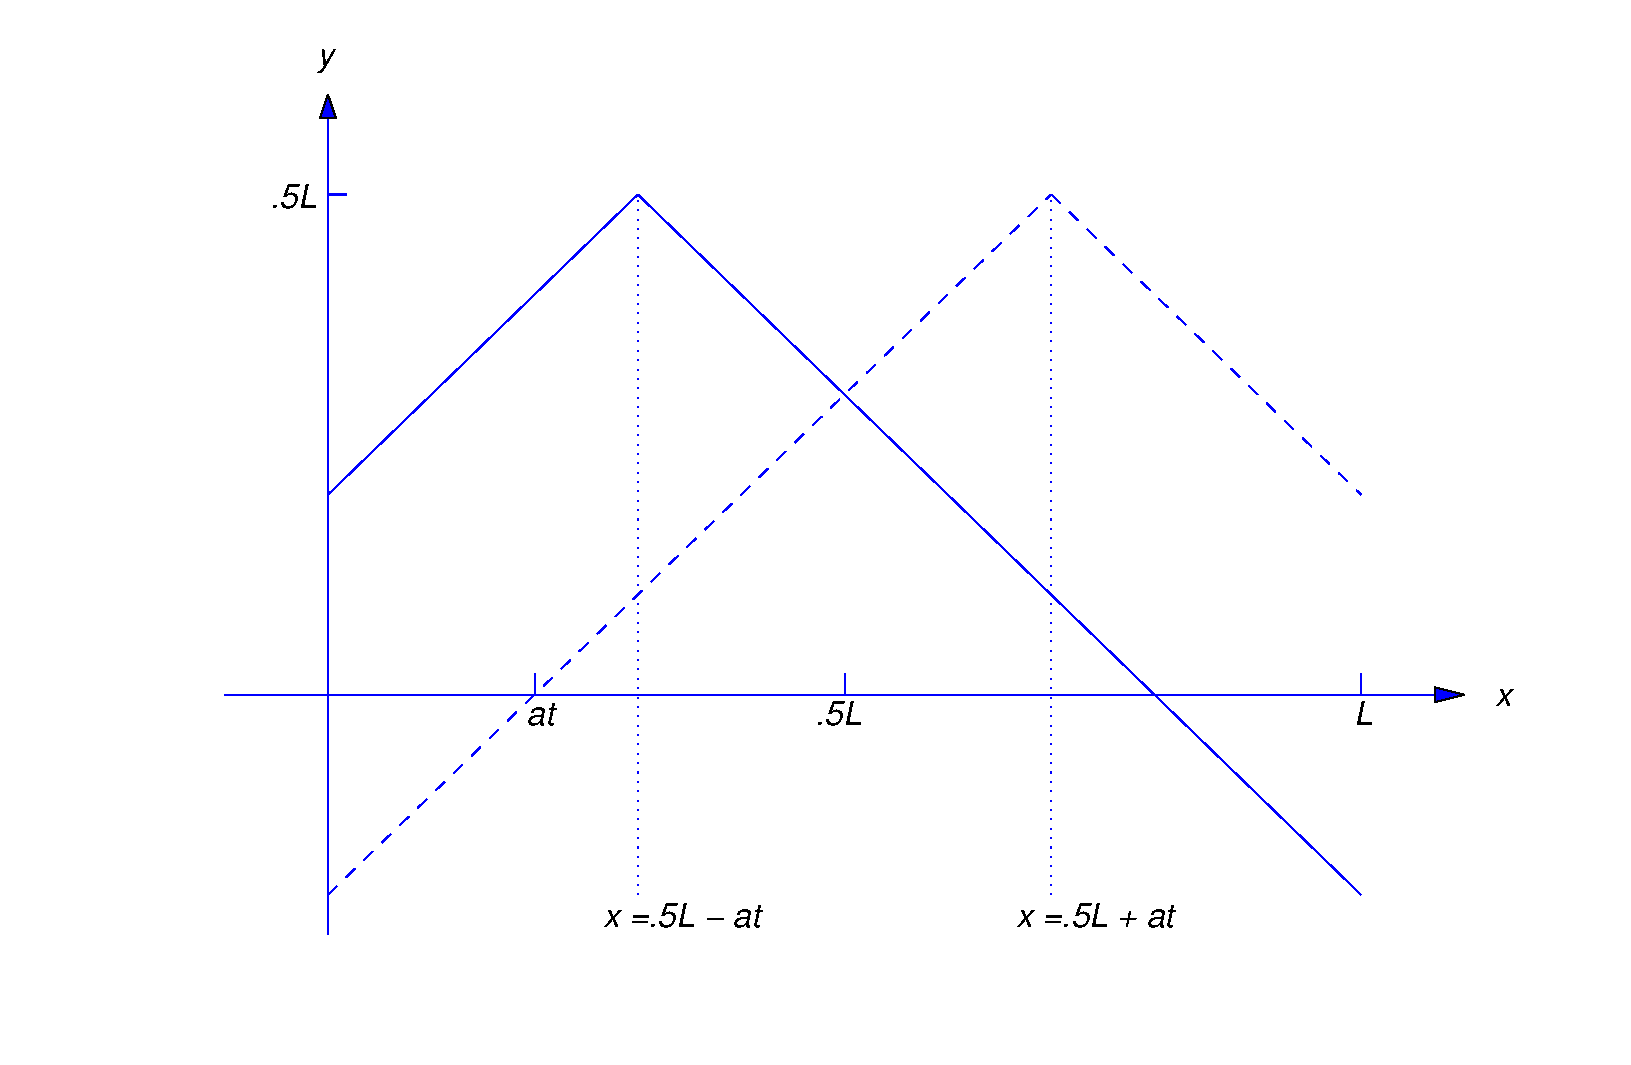
\includegraphics[bb=-78 148 689 643,width=5.67in,height=3.66in,keepaspectratio]{fig120210}}
\caption{ The part of the graph from Figure~\ref{figure:12.2.9} on $[0,L]$}
  \label{figure:12.2.10}
\end{minipage}
  \begin{minipage}[b]{0.5\linewidth}
    \centering
   \scalebox{.65}{
  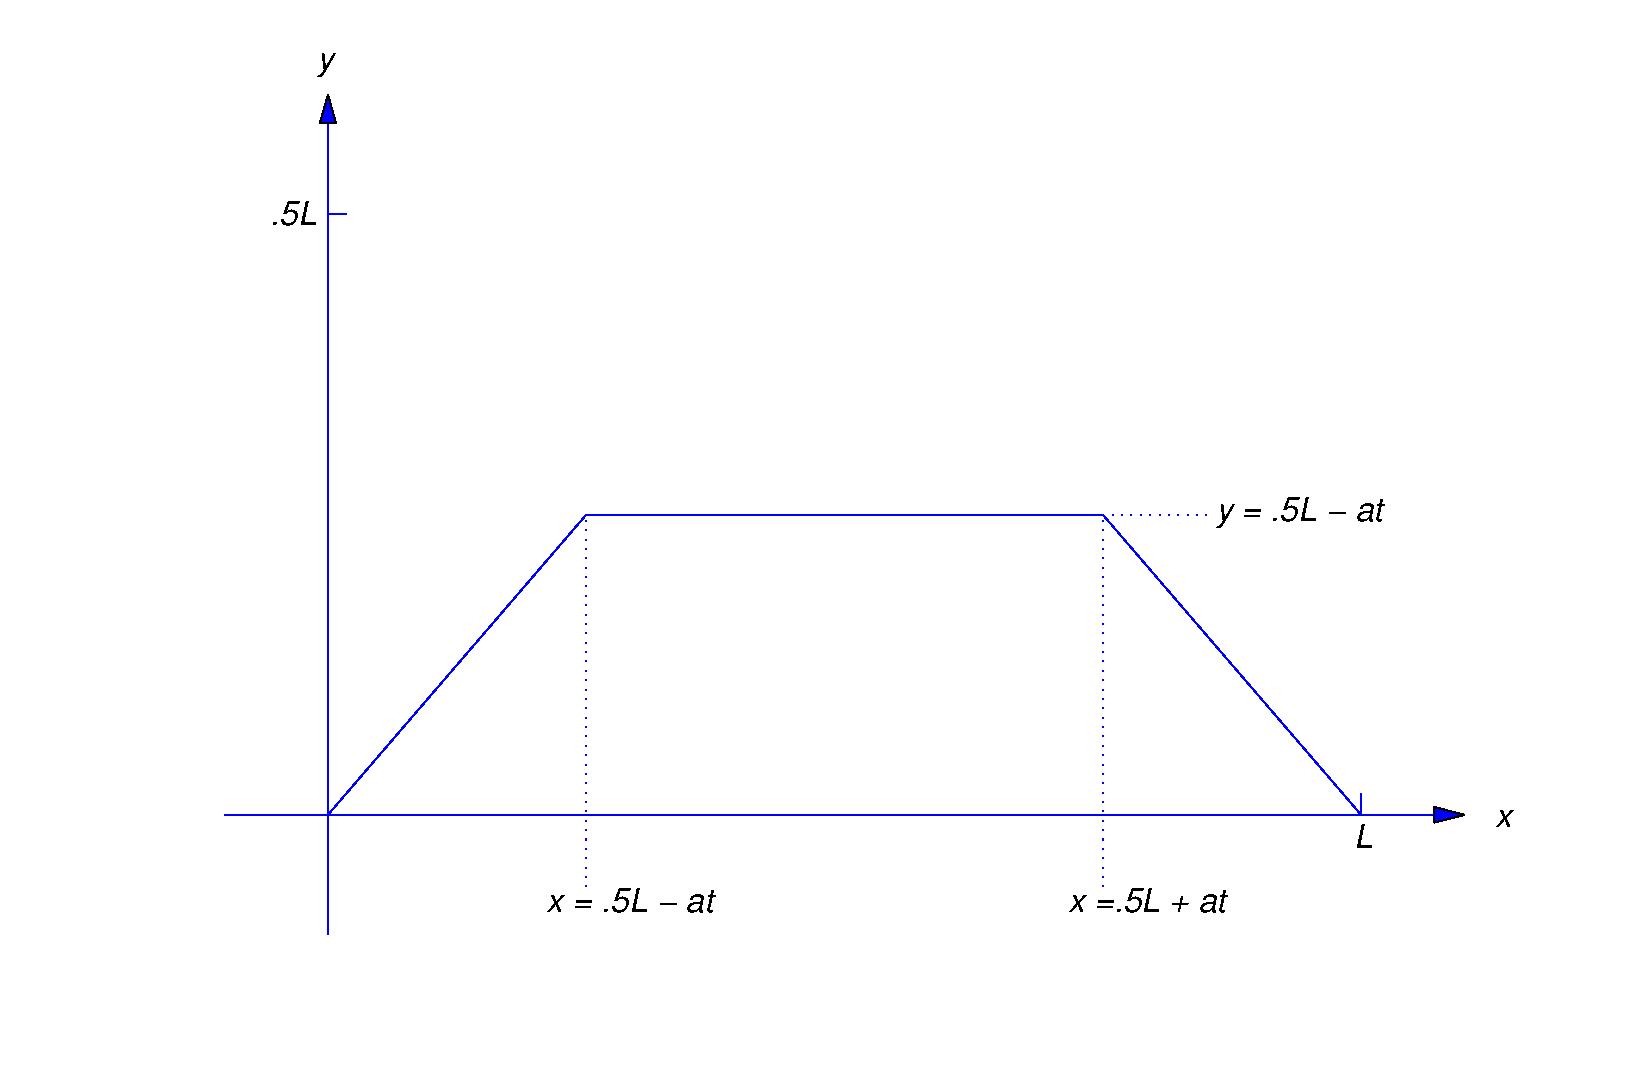
\includegraphics[bb=-78 148 689 643,width=5.67in,height=3.66in,keepaspectratio]{fig120211}}
\caption{ The graph of \eqref{eq:12.2.23} on $[0,L]$ for a fixed $t$ in
$(0,L/2a)$}
  \label{figure:12.2.11}
\end{minipage}
\end{figure}

\technology
\medskip

Although the formal solution
$$
u(x,t)=\sum_{n=1}^\infty\left(\alpha_n\cos{n\pi at\over
L}+{\beta_nL\over n\pi a}\sin{n\pi at\over L}\right)
\sin{n\pi x\over L}
$$
of \eqref{eq:12.2.1} is defined for all $(x,t)$, we're mainly interested
in its behavior for $0\le x\le L$ and $t\ge0$. In fact, it's
sufficient to consider only values of $t$ in the interval $0\le
t<2L/a$, since
$$
u(x,t+2kL/a)=u(x,t)
$$
for all $(x,t)$  if $k$ is an integer. (Verify.)

You can create an animation of the motion of the string
by performing the following numerical experiment.

Let $m$  and $k$ be positive integers. Let
$$
t_j={2Lj\over ka},\quad j=0,1,\dots k;
$$
thus, $t_0$, $t_1$, \dots $t_k$ are equally spaced points in $[0,2L/a]$.
For each $j=0$, $1$ ,$2$, \dots $k$, graph the partial sum
$$
u_m(x,t_j)=\sum_{n=1}^m\left(\alpha_n\cos{n\pi at_j\over
L}+{\beta_nL\over n\pi a}\sin{n\pi at_j\over L}\right)
\sin{n\pi x\over L}
$$
on $[0,L]$ as a function of $x$.  Write your program so that
each graph remains displayed on the monitor for a short time,
and is then deleted and replaced by the next. Repeat this
procedure for various values of $m$ and $k$.

We suggest that you perform experiments of this kind in the exercises
marked \Cex\hspace*{-3pt}, without other specific instructions. (These
exercises
were chosen arbitrarily;   the experiment is worthwhile in all the
exercises dealing with specific initial-boundary value problems.) In
some of the exercises the formal solutions have other forms, defined
in Exercises~\ref{exer:12.2.17}, \ref{exer:12.2.34}, and
\ref{exer:12.2.49};     however,
the idea of the experiment is the same.

\exercises
\noindent

\noindent
{\it In Exercises~\ref{exer:12.2.1}-\ref{exer:12.2.15} solve the
initial-boundary value problem.
In some of these exercises, Theorem~\ref{thmtype:11.3.5}\part{b}
or Exercise~$11.3$.~\hspace*{-3pt}\ref{exer:11.3.35} will
simplify the computation of the coefficients in the Fourier sine series.}

\begin{exerciselist}

\item\label{exer:12.2.1}
$u_{tt}=9u_{xx},\quad 0<x<1,\quad t>0$,\\
$u(0,t)=0,\quad u(1,t)=0,\quad t>0$,\\
$u(x,0)=0,\quad
 u_t(x,0)=
\left\{\begin{array}{cl}
x,&0\le x\le{1\over2},\\1-x,&{1\over2}\le x\le1
\end{array}\right.,\quad0\le x\le1$

\item\label{exer:12.2.2}
$u_{tt}=9u_{xx},\quad 0<x<1,\quad t>0$,\\
$u(0,t)=0,\quad u(1,t)=0,\quad t>0$,\\
$u(x,0)=x(1-x),\quad u_t(x,0)=0,\quad0\le x\le 1$

\item\label{exer:12.2.3}
$u_{tt}=7u_{xx},\quad 0<x<1,\quad t>0$,\\
$u(0,t)=0,\quad u(1,t)=0,\quad t>0$,\\
$u(x,0)=x^2(1-x),\quad u_t(x,0)=0,\quad0\le x\le1$

\item\label{exer:12.2.4}  \Cex
$u_{tt}=9u_{xx},\quad 0<x<1,\quad t>0$,\\
$u(0,t)=0,\quad u(1,t)=0,\quad t>0$,\\
$u(x,0)=0,\quad u_t(x,0)=x(1-x),\quad0\le x\le 1$

\item\label{exer:12.2.5}
$u_{tt}=7u_{xx},\quad 0<x<1,\quad t>0$,\\
$u(0,t)=0,\quad u(1,t)=0,\quad t>0$,\\
$u(x,0)=0\quad u_t(x,0)=x^2(1-x),\quad0\le x\le1$

\item\label{exer:12.2.6}
$u_{tt}=64u_{xx},\quad 0<x<3,\quad t>0$,\\
$u(0,t)=0,\quad u(3,t)=0,\quad t>0$,\\
$u(x,0)=x(x^2-9),\quad u_t(x,0)=0,\quad0\le x\le 3$

\item\label{exer:12.2.7}
$u_{tt}=4u_{xx},\quad 0<x<1,\quad t>0$,\\
$u(0,t)=0,\quad u(1,t)=0,\quad t>0$,\\
$u(x,0)=x(x^3-2x^2+1),\quad u_t(x,0)=0,\quad0\le x\le1$

\item\label{exer:12.2.8}  \Cex
$u_{tt}=64u_{xx},\quad 0<x<3,\quad t>0$,\\
  $u(0,t)=0,\quad u(3,t)=0,\quad t>0$,\\
$u(x,0)=0,\quad u_t(x,0)=x(x^2-9),\quad0\le x\le 3$

\item\label{exer:12.2.9}
$u_{tt}=4u_{xx},\quad 0<x<1,\quad t>0$,\\
$u(0,t)=0,\quad u(1,t)=0,\quad t>0$,\\
$u(x,0)=0,\quad u_t(x,0)=x(x^3-2x^2+1),\quad0\le x\le1$

\item\label{exer:12.2.10}
$u_{tt}=5u_{xx},\quad 0<x<\pi,\quad t>0$,\\
$u(0,t)=0,\quad u(\pi,t)=0,\quad t>0$,\\
$u(x,0)=x\sin x,\quad u_t(x,0)=0,\quad0\le x\le \pi$

\item\label{exer:12.2.11}
$u_{tt}=u_{xx},\quad 0<x<1,\quad t>0$,\\
$u(0,t)=0,\quad u(1,t)=0,\quad t>0$,\\
$u(x,0)=x(3x^4-5x^3+2),\quad u_t(x,0)=0,\quad0\le x\le1$

\item\label{exer:12.2.12}   \Cex
$u_{tt}=5u_{xx},\quad 0<x<\pi,\quad t>0$,\\
$u(0,t)=0,\quad u(\pi,t)=0,\quad t>0$,\\
$u(x,0)=0,\quad u_t(x,0)=x\sin x,\quad0\le x\le \pi$

\item\label{exer:12.2.13}
$u_{tt}=u_{xx},\quad 0<x<1,\quad t>0$,\\
$u(0,t)=0,\quad u(1,t)=0,\quad t>0$,\\
$u(x,0)=0,\quad u_t(x,0)=x(3x^4-5x^3+2),\quad0\le x\le1$

\item\label{exer:12.2.14}
$u_{tt}=9u_{xx},\quad 0<x<1,\quad t>0$,\\
$u(0,t)=0,\quad u(1,t)=0,\quad t>0$,\\
$u(x,0)=x(3x^4-10x^2+7),\quad u_t(x,0)=0,\quad0\le x\le1$

\item\label{exer:12.2.15}   \Cex
$u_{tt}=9u_{xx},\quad 0<x<1,\quad t>0$,\\
$u(0,t)=0,\quad u(1,t)=0,\quad t>0$,\\
$u(x,0)=0\quad u_t(x,0)=x(3x^4-10x^2+7),\quad0\le x\le1$

\item\label{exer:12.2.16}
We saw
that the displacement of the plucked string is,
on the one hand,
$$
u(x,t)=\dst{4L\over\pi^2}\sum_{n=1}^\infty{(-1)^{n+1}\over(2n-1)^2}
\cos{(2n-1)\pi at\over L}\sin{(2n-1)\pi x\over L},\; 0\le x\le
L,\; t\ge 0,
\eqno{\rm(A)}
$$
and, on the other hand,
$$
u(x,\tau)=
\left\{\begin{array}{cl}
x,&0\le x\le{L\over2}-a\tau,\\[2\jot]
{L\over2}-a\tau,&{L\over2}-a\tau\le x\le{L\over2}+a\tau,\\[2\jot]
L-x,&{L\over2}-a\tau\le x\le L.
\end{array}\right.
\eqno{\rm(B)}
$$
if $0\le \tau\le L/2a$.
The first objective  of this exercise is to show that (B) can be used
to compute $u(x,t)$ for  $0\le x\le L$ and all $t>0$.
\begin{alist}
\item % (a)
Show that if $t>0$,  there's a nonnegative integer
$m$ such that either
$$
\mbox{\bf(i)}\quad t={mL\over a}+\tau\mbox{\quad or \quad}
\mbox{\bf(ii)}\quad t={(m+1)L\over a}-\tau,
$$
where $0\le \tau\le L/2a$.
\item % (b)
Use (A) to show that $u(x,t)=(-1)^mu(x,\tau)$ if \part{i}
holds, while $u(x,t)=(-1)^{m+1}u(x,\tau)$ if \part{ii} holds.
\item % (c)
\Lex\;  Perform the following experiment for specific values
of $L$ and $a$ and various values of $m$ and $k$:
 Let
$$
t_j={Lj\over 2ka},\quad j=0,1,\dots k;
$$
thus, $t_0$, $t_1$, \dots, $t_k$ are equally spaced points in $[0,L/2a]$.
For each $j=0$, $1$ , $2$,\dots, $k$, graph the $m$th partial sum
of (A) and $u(x,t_j)$ computed from (B) on the same axis.
Create an animation, as described in the remarks on using
technology at the end of the section.
\end{alist}

\item\label{exer:12.2.17}
If a string vibrates with the end at $x=0$ free to move in a
frictionless
vertical track and the end at $x=L$ fixed, then the initial-boundary
value problem for its displacement takes the form
$$
\begin{array}{c}
u_{tt}=a^2u_{xx},\quad 0<x<L,\quad t>0,\\
 u_x(0,t)=0,\quad u(L,t)=0,\quad t>0,\\
u(x,0)=f(x),\quad u_t(x,0)=g(x),\quad 0\le x\le L.
\end{array}
\eqno{\rm(A)}
$$
Justify defining the formal solution of (A) to be
$$
u(x,t)=\sum_{n=1}^\infty
\left(\alpha_n\cos{(2n-1)\pi a
t\over2L}+{2L\beta_n\over(2n-1)\pi a}\sin{(2n-1)\pi
at\over2L}\right)
\cos{(2n-1)\pi
x\over2L},
$$
where
$$
C_{M\!f}(x)=\sum_{n=1}^\infty\alpha_n\cos{(2n-1)\pi x\over2L}
\mbox{\quad and \quad}
C_{M\!g}(x)=\sum_{n=1}^\infty\beta_n\cos{(2n-1)\pi x\over2L}
$$
are the mixed Fourier cosine series of $f$ and $g$
on $[0,L]$; that is,
$$
\alpha_n={2\over L}\int_0^Lf(x)\cos{(2n-1)\pi x\over2L}\,dx
\mbox{\quad and \quad}
\beta_n={2\over L}\int_0^Lg(x)\cos{(2n-1)\pi x\over2L}\,dx.
$$

\exercisetext{
In Exercises~\ref{exer:12.2.18}-\ref{exer:12.2.31}, use
Exercise~\ref{exer:12.2.17} to solve the initial-boundary
value problem.  In some of these exercises
Theorem~\ref{thmtype:11.3.5}\part{c}
or Exercise~$11.3$.~\hspace*{-3pt}\ref{exer:11.3.42}\part{b} will simplify
the
computation of the coefficients in the mixed Fourier cosine series.}

\item\label{exer:12.2.18}
$u_{tt}=9u_{xx},\quad 0<x<2,\quad t>0$,\\
$u_x(0,t)=0,\quad u(2,t)=0,\quad t>0$,\\
$u(x,0)=4-x^2,\quad u_t(x,0)=0,\quad0\le x\le2$

\item\label{exer:12.2.19}
$u_{tt}=4u_{xx},\quad 0<x<1,\quad t>0$,\\
$u_x(0,t)=0,\quad u(1,t)=0,\quad t>0$,\\
$u(x,0)=x^2(1-x),\quad u_t(x,0)=0,\quad0\le x\le 1$

\item\label{exer:12.2.20}
$u_{tt}=9u_{xx},\quad 0<x<2,\quad t>0$,\\
$u_x(0,t)=0,\quad u(2,t)=0,\quad t>0$,\\
$u(x,0)=0,\quad u_t(x,0)=4-x^2,\quad0\le x\le2$

\item\label{exer:12.2.21}
$u_{tt}=4u_{xx},\quad 0<x<1,\quad t>0$,\\
$u_x(0,t)=0,\quad u(1,t)=0,\quad t>0$,\\
$u(x,0)=0,\quad u_t(x,0)=x^2(1-x),\quad0\le x\le 1$

\item\label{exer:12.2.22}  \Cex
$u_{tt}=5u_{xx},\quad 0<x<1,\quad t>0$,\\
$u_x(0,t)=0,\quad u(1,t)=0,\quad t>0$,\\
$u(x,0)=2x^3+3x^2-5,\quad u_t(x,0)=0,\quad0\le x\le1$

\item\label{exer:12.2.23}
$u_{tt}=3u_{xx},\quad 0<x<\pi,\quad t>0$,\\
$u_x(0,t)=0,\quad u(\pi,t)=0,\quad t>0$,\\
$u(x,0)=\pi^3-x^3,\quad u_t(x,0)=0,\quad0\le x\le\pi$

\item\label{exer:12.2.24}
$u_{tt}=5u_{xx},\quad 0<x<1,\quad t>0$,\\
$u_x(0,t)=0,\quad u(1,t)=0,\quad t>0$,\\
$u(x,0)=0,\quad u_t(x,0)=2x^3+3x^2-5,\quad0\le x\le1$

\item\label{exer:12.2.25}   \Cex
$u_{tt}=3u_{xx},\quad 0<x<\pi,\quad t>0$,\\
$u_x(0,t)=0,\quad u(\pi,t)=0,\quad t>0$,\\
$u(x,0)=0,\quad u_t(x,0)=\pi^3-x^3,\quad0\le x\le\pi$

\item\label{exer:12.2.26}
$u_{tt}=9u_{xx},\quad 0<x<1,\quad t>0$,\\
$u_x(0,t)=0,\quad u(1,t)=0,\quad t>0$,\\
$u(x,0)=x^4-2x^3+1,\quad u_t(x,0)=0,\quad0\le x\le1$

\item\label{exer:12.2.27}
$u_{tt}=7u_{xx},\quad 0<x<1,\quad t>0$,\\
$u_x(0,t)=0,\quad u(1,t)=0,\quad t>0$,\\
$u(x,0)=4x^3+3x^2-7,\quad u_t(x,0)=0,\quad0\le x\le1$

\item\label{exer:12.2.28}
$u_{tt}=9u_{xx},\quad 0<x<1,\quad t>0$,\\
$u_x(0,t)=0,\quad u(1,t)=0,\quad t>0$,\\
$u(x,0)=0,\quad u_t(x,0)=x^4-2x^3+1,\quad0\le x\le1$

\item\label{exer:12.2.29}   \Cex
$u_{tt}=7u_{xx},\quad 0<x<1,\quad t>0$,\\
$u_x(0,t)=0,\quad u(1,t)=0,\quad t>0$,\\
$u(x,0)=0,\quad u_t(x,0)=4x^3+3x^2-7,\quad0\le x\le1$

\item\label{exer:12.2.30}
$u_{tt}=u_{xx},\quad 0<x<1,\quad t>0$,\\
$u_x(0,t)=0,\quad u(1,t)=0,\quad t>0$,\\
$u(x,0)=x^4-4x^3+6x^2-3,\quad u_t(x,0)=0,\quad0\le x\le1$

\item\label{exer:12.2.31}
$u_{tt}=u_{xx},\quad 0<x<1,\quad t>0$,\\
$u_x(0,t)=0,\quad u(1,t)=0,\quad t>0$,\\
$u(x,0)=0,\quad u_t(x,0)=x^4-4x^3+6x^2-3,\quad0\le x\le1$

\item\label{exer:12.2.32} Adapt the proof of Theorem~\ref{thmtype:12.2.2}
to find d'Alembert's solution of the initial-boundary value problem
in Exercise~\ref{exer:12.2.17}.

\item\label{exer:12.2.33}
Use the result of Exercise~\ref{exer:12.2.32} to show that the formal
solution of the initial-boundary value problem in
Exercise~\ref{exer:12.2.17}
is an actual solution if $g$ is differentiable and $f$ is twice
differentiable on $[0,L]$ and
$$
g'_+(0)=g(L)=f'_+(0)=f(L)=f''_-(L)=0.
$$
\hint{See Exercise~$11.3$.~\hspace*{-3pt}\ref{exer:11.3.57},
and apply Theorem~\ref{thmtype:12.2.3} with
$L$ replaced by $2L$.}

\item\label{exer:12.2.34}
Justify  defining the formal solution of the initial-boundary
value problem
$$
\begin{array}{c}
u_{tt}=a^2u_{xx},\quad 0<x<L,\quad t>0,\\
 u(0,t)=0,\quad u_x(L,t)=0,\quad t>0,\\
u(x,0)=f(x),\quad u_t(x,0)=g(x),\quad 0\le x\le L
\end{array}
$$
to be
$$
u(x,t)=\sum_{n=1}^\infty
\left(\alpha_n\cos{(2n-1)\pi a
t\over2L}+{2L\beta_n\over(2n-1)\pi a}\sin{(2n-1)\pi
at\over2L}\right)
\sin{(2n-1)\pi x\over2L},
$$
where
$$
S_{M\!f}(x)=\sum_{n=1}^\infty\alpha_n\sin{(2n-1)\pi x\over2L}
\mbox{\quad and \quad}
S_{M\!g}(x)=\sum_{n=1}^\infty\beta_n\sin{(2n-1)\pi x\over2L}
$$
are the mixed Fourier sine series of $f$ and $g$
on $[0,L]$; that is,
$$
\alpha_n={2\over L}\int_0^Lf(x)\sin{(2n-1)\pi x\over2L}\,dx
\mbox{\quad and \quad}
\beta_n={2\over L}\int_0^Lg(x)\sin{(2n-1)\pi x\over2L}\,dx.
$$

\exercisetext{
In Exercises~\ref{exer:12.2.35}-\ref{exer:12.2.46} use
Exercise~\ref{exer:12.2.34} to solve the initial-boundary
value problem.  In some of these exercises
Theorem~\ref{thmtype:11.3.5}\part{d}
or Exercise~$11.3$.~\hspace*{-3pt}\ref{exer:11.3.50}\part{b} will simplify
the
computation of the coefficients in the mixed Fourier sine series.}

\item\label{exer:12.2.35}
$u_{tt}=64u_{xx},\quad 0<x<\pi,\quad t>0$,\\
$u(0,t)=0,\quad u_x(\pi,t)=0,\quad t>0$,\\
$u(x,0)=x(2\pi-x),\quad u_t(x,0)=0,\quad0\le x\le \pi$

\item\label{exer:12.2.36}
$u_{tt}=9u_{xx},\quad 0<x<1,\quad t>0$,\\
$u(0,t)=0,\quad u_x(1,t)=0,\quad t>0$,\\
$u(x,0)=x^2(3-2x),\quad u_t(x,0)=0,\quad0\le x\le 1$

\item\label{exer:12.2.37}
$u_{tt}=64u_{xx},\quad 0<x<\pi,\quad t>0$,\\
$u(0,t)=0,\quad u_x(\pi,t)=0,\quad t>0$,\\
$u(x,0)=0,\quad u_t(x,0)=x(2\pi-x),\quad0\le x\le \pi$

\item\label{exer:12.2.38}   \Cex
$u_{tt}=9u_{xx},\quad 0<x<1,\quad t>0$,\\
$u(0,t)=0,\quad u_x(1,t)=0,\quad t>0$,\\
$u(x,0)=0,\quad u_t(x,0)=x^2(3-2x),\quad0\le x\le 1$

\item\label{exer:12.2.39}
$u_{tt}=9u_{xx},\quad 0<x<1,\quad t>0$,\\
$u(0,t)=0,\quad u_x(1,t)=0,\quad t>0$,\\
$u(x,0)=(x-1)^3+1,\quad u_t(x,0)=0,\quad0\le x\le 1$

\item\label{exer:12.2.40}
$u_{tt}=3u_{xx},\quad 0<x<\pi,\quad t>0$,\\
$u(0,t)=0,\quad u_x(\pi,t)=0,\quad t>0$,\\
$u(x,0)=x(x^2-3\pi^2),\quad u_t(x,0)=0,\quad0\le x\le\pi$

\item\label{exer:12.2.41}
$u_{tt}=9u_{xx},\quad 0<x<1,\quad t>0$,\\
$u(0,t)=0,\quad u_x(1,t)=0,\quad t>0$,\\
$u(x,0)=0,\quad u_t(x,0)=(x-1)^3+1,\quad0\le x\le 1$

\item\label{exer:12.2.42}
$u_{tt}=3u_{xx},\quad 0<x<\pi,\quad t>0$,\\
$u(0,t)=0,\quad u_x(\pi,t)=0,\quad t>0$,\\
$u(x,0)=0,\quad u_t(x,0)=x(x^2-3\pi^2),\quad0\le x\le\pi$

\item\label{exer:12.2.43}
$u_{tt}=5u_{xx},\quad 0<x<1,\quad t>0$,\\
$u(0,t)=0,\quad u_x(1,t)=0,\quad t>0$,\\
$u(x,0)=x^3(3x-4),\quad u_t(x,0)=0,\quad0\le x\le1$

\item\label{exer:12.2.44} \Cex
$u_{tt}=16u_{xx},\quad 0<x<1,\quad t>0$,\\
$u(0,t)=0,\quad u_x(1,t)=0,\quad t>0$,\\
$u(x,0)=x(x^3-2x^2+2),\quad u_t(x,0)=0,\quad0\le x\le1$

\item\label{exer:12.2.45}
$u_{tt}=5u_{xx},\quad 0<x<1,\quad t>0$,\\
$u(0,t)=0,\quad u_x(1,t)=0,\quad t>0$,\\
$u(x,0)=0,\quad u_t(x,0)=x^3(3x-4),\quad0\le x\le1$

\item\label{exer:12.2.46}  \Cex
$u_{tt}=16u_{xx},\quad 0<x<1,\quad t>0$,\\
$u(0,t)=0,\quad u_x(1,t)=0,\quad t>0$,\\
$u(x,0)=0,\quad u_t(x,0)=x(x^3-2x^2+2),\quad0\le x\le1$

\item\label{exer:12.2.47} Adapt the proof of Theorem~\ref{thmtype:12.2.2}
to find d'Alembert's solution of the initial-boundary value problem
in Exercise~\ref{exer:12.2.34}.

\item\label{exer:12.2.48}
Use the result of Exercise~\ref{exer:12.2.47} to show that the formal
solution of the initial-boundary value problem in
Exercise~\ref{exer:12.2.34}
is an actual solution if $g$ is differentiable and $f$ is twice
differentiable on $[0,L]$ and
$$
f(0)=f'_-(L)=g(0)=g_-'(L)=f''_+(0)=0.
$$
\hint{See Exercise~$11.3$.~\hspace*{-3pt}\ref{exer:11.3.58}
and apply Theorem~\ref{thmtype:12.2.3} with
$L$ replaced by $2L$.}

\item\label{exer:12.2.49}
Justify  defining the formal solution of the initial-boundary
value problem
$$
\begin{array}{c}
u_{tt}=a^2u_{xx},\quad 0<x<L,\quad t>0,\\
 u_x(0,t)=0,\quad u_x(L,t)=0,\quad t>0,\\
u(x,0)=f(x),\quad u_t(x,0)=g(x),\quad 0\le x\le L.
\end{array}
$$
to be
$$
u(x,t)=\alpha_0+\beta_0t+\sum_{n=1}^\infty
\left(\alpha_n\cos{n\pi at\over L}+{L\beta_n\over n\pi
a}\sin{n\pi at\over L}\right)
\cos{n\pi x\over L},
$$
where
$$
C_f(x)=\alpha_0+\sum_{n=1}^\infty\alpha_n\cos{n\pi x\over L}
\mbox{\quad and \quad}
C_g(x)=\beta_0+\sum_{n=1}^\infty\beta_n\cos{n\pi x\over L}
$$
are the Fourier cosine series of $f$ and $g$
on $[0,L]$; that is,
$$
\alpha_0={1\over L}\int_0^Lf(x)\,dx,\quad
\beta_0={1\over L}\int_0^Lg(x)\,dx,
$$
$$
\alpha_n={2\over L}\int_0^Lf(x)\cos{n\pi x\over L}\,dx,
\mbox{\quad and \quad}
\beta_n={2\over L}\int_0^Lg(x)\cos{n\pi x\over L}\,dx,\quad
n=1,2,3,\dots.
$$

\exercisetext{
In Exercises~\ref{exer:12.2.50}-\ref{exer:12.2.59} use
Exercise~\ref{exer:12.2.49} to solve
the initial-boundary value problem. In some of these exercises
Theorem~\ref{thmtype:11.3.5}\part{a}
 will simplify the computation
of the coefficients in the  Fourier cosine series.}

\item\label{exer:12.2.50}
$u_{tt}=5u_{xx},\quad 0<x<2,\quad t>0$,\\
$u_x(0,t)=0,\quad u_x(2,t)=0,\quad t>0$,\\
$u(x,0)=2x^2(3-x),\quad u_t(x,0)=0,\quad0\le x\le 2$

\item\label{exer:12.2.51}
$u_{tt}=5u_{xx},\quad 0<x<2,\quad t>0$,\\
$u_x(0,t)=0,\quad u_x(2,t)=0,\quad t>0$,\\
$u(x,0)=0,\quad u_t(x,0)=2x^2(3-x),\quad0\le x\le 2$

\item\label{exer:12.2.52}
$u_{tt}=4u_{xx},\quad 0<x<\pi,\quad t>0$,\\
$u_x(0,t)=0,\quad u_x(\pi,t)=0,\quad t>0$,\\
$u(x,0)=x^3(3x-4\pi),\quad u_t(x,0)=0,\quad0\le x\le \pi$

\item\label{exer:12.2.53}
$u_{tt}=7u_{xx},\quad 0<x<1,\quad t>0$,\\
$u_x(0,t)=0,\quad u_x(1,t)=0,\quad t>0$,\\
$u(x,0)=3x^2(x^2-2),\quad u_t(x,0)=0,\quad0\le x\le 1$

\item\label{exer:12.2.54}  \Cex
$u_{tt}=4u_{xx},\quad 0<x<\pi,\quad t>0$,\\
$u_x(0,t)=0,\quad u_x(\pi,t)=0,\quad t>0$,\\
$u(x,0)=0,\quad u_t(x,0)=x^3(3x-4\pi),\quad0\le x\le \pi$

\item\label{exer:12.2.55}
$u_{tt}=7u_{xx},\quad 0<x<1,\quad t>0$,\\
$u_x(0,t)=0,\quad u_x(1,t)=0,\quad t>0$,\\
$u(x,0)=0,\quad u_t(x,0)=3x^2(x^2-2),\quad0\le x\le 1$

\item\label{exer:12.2.56}
$u_{tt}=16u_{xx},\quad 0<x<\pi,\quad t>0$,\\
$u_x(0,t)=0,\quad u_x(\pi,t)=0,\quad t>0$,\\
$u(x,0)=x^2(x-\pi)^2,\quad u_t(x,0)=0,\quad0\le x\le \pi$

\item\label{exer:12.2.57}  \Cex
$u_{tt}=u_{xx},\quad 0<x<1,\quad t>0$,\\
$u_x(0,t)=0,\quad u_x(1,t)=0,\quad t>0$,\\
$u(x,0)=x^2(3x^2-8x+6),\quad u_t(x,0)=0,\quad0\le x\le 1$

\item\label{exer:12.2.58}
$u_{tt}=16u_{xx},\quad 0<x<\pi,\quad t>0$,\\
$u_x(0,t)=0,\quad u_x(\pi,t)=0,\quad t>0$,\\
$u(x,0)=0,\quad u_t(x,0)=x^2(x-\pi)^2,\quad0\le x\le \pi$

\item\label{exer:12.2.59}   \Cex
$u_{tt}=u_{xx},\quad 0<x<1,\quad t>0$,\\
$u_x(0,t)=0,\quad u_x(1,t)=0,\quad t>0$,\\
$u(x,0)=0,\quad u_t(x,0)=x^2(3x^2-8x+6),\quad0\le x\le 1$

\item\label{exer:12.2.60} Adapt the proof of Theorem~\ref{thmtype:12.2.2}
to find d'Alembert's solution of the initial-boundary value problem
in Exercise~\ref{exer:12.2.49}.

\item\label{exer:12.2.61}
Use the result of Exercise~\ref{exer:12.2.60} to show that the formal
solution of the initial-boundary value problem in
Exercise~\ref{exer:12.2.49}
is an actual solution if $g$ is differentiable and $f$ is twice
differentiable on $[0,L]$ and
$$
f'_+(0)=f'_-(L)=g'_+(0)=g_-'(L)=0.
$$

\item\label{exer:12.2.62}
Suppose $\lambda$ and $\mu$ are constants and either $p_n(x)=
\cos n\lambda x$ or $p_n(x)=\sin n\lambda x$, while either
$q_n(t)=\cos n\mu t$ or $q_n(t)=\sin n\mu t$ for $n=1$, $2$, $3$, \dots.
Let
$$
u(x,t)=\sum_{n=1}^\infty k_np_n(x)q_n(t),
\eqno{\rm(A)}
$$
where $\{k_n\}_{n=1}^\infty$ are constants.
\begin{alist}
\item % (a)
Show that if $\sum_{n=1}^\infty |k_n|$ converges
then $u(x,t)$ converges for all $(x,t)$.
\item % (b)
Use Theorem~12.1.2 to
show that if $\sum_{n=1}^\infty n|k_n|$ converges then
(A) can be differentiated term by term with respect to $x$
and $t$ for all $(x,t)$; that is,
$$
u_x(x,t)=
\sum_{n=1}^\infty k_np_n'(x)q_n(t)
$$
and
$$
u_t(x,t)=
\sum_{n=1}^\infty k_np_n(x)q_n'(t).
$$
\item % (c)
Suppose  $\sum_{n=1}^\infty n^2|k_n|$ converges. Show that
$$
u_{xx}(x,y)=
\sum_{n=1}^\infty k_np_n''(x)q_n(t)
$$
and
$$
u_{tt}(x,y)=
\sum_{n=1}^\infty k_np_n(x)q_n''(t)
$$
\item % (d)
Suppose  $\sum_{n=1}^\infty n^2|\alpha_n|$ and
$\sum_{n=1}^\infty n|\beta_n|$ both converge.
Show that the formal solution
$$
u(x,t)=\sum_{n=1}^\infty\left(\alpha_n\cos{n\pi at\over
L}+{\beta_nL\over n\pi a}\sin{n\pi at\over L}\right)
\sin{n\pi x\over L}
$$
of Equation~\ref{eq:12.2.1} satisfies
$u_{tt}=a^2u_{xx}$ for all
$(x,t)$.

This conclusion also applies to the formal solutions defined in
Exercises~\ref{exer:12.2.17}, \ref{exer:12.2.34}, and \ref{exer:12.2.49}.
\end{alist}

\item\label{exer:12.2.63}
Suppose $g$ is differentiable and $f$ is twice differentiable on
$(-\infty,\infty)$, and let
$$
u_0(x,t)={f(x+at)+f(x-at)\over2}\mbox{\quad and \quad}
u_1(x,t)={1\over2a}\int_{x-at}^{x+at}g(u)\,du.
$$
\begin{alist}
\item % (a)
Show that
$$
{\partial^2 u_0\over\partial t^2}=a^2{\partial^2u_0\over\partial
x^2},\quad-\infty<x<\infty,\quad t>0,
$$
and
$$
u_0(x,0)=f(x),\quad  {\partial u_0\over\partial t}(x,0)=0,\quad
-\infty<x<\infty.
$$
\item % (b)
Show that
$$
{\partial^2 u_1\over\partial t^2}=a^2{\partial^2u_1\over\partial
x^2},\quad-\infty<x<\infty,\quad t>0,
$$
and
$$
u_1(x,0)=0,\quad  {\partial u_1\over\partial t}(x,0)=g(x),\quad
-\infty<x<\infty.
$$
\item % (c)
Solve
$$
u_{tt}=a^2u_{xx},\quad-\infty<t<\infty,\quad t>0,
$$
$$
u(x,0)=f(x),\quad u_t(x,0)=g(x),\quad-\infty<x<\infty.
$$
\end{alist}

\exercisetext{In Exercises~\ref{exer:12.2.64}-\ref{exer:12.2.68} use the
result of Exercise~\ref{exer:12.2.63} to find a solution of
$$
u_{tt}=a^2u_{xx},\quad -\infty<x<\infty
$$
that satisfies the given initial conditions.}

\item\label{exer:12.2.64}
$u(x,0)=x$,\quad $u_t(x,0)=4ax$,\quad $-\infty<x<\infty$

\item\label{exer:12.2.65}
$u(x,0)=x^2$,\quad $u_t(x,0)=1$,\quad $-\infty<x<\infty$

\item\label{exer:12.2.66}
$u(x,0)=\sin x$,\quad $u_t(x,0)=a\cos x$,\quad $-\infty<x<\infty$

\item\label{exer:12.2.67}
$u(x,0)=x^3$,\quad $u_t(x,0)=6x^2$,\quad $-\infty<x<\infty$

\item\label{exer:12.2.68}
$u(x,0)=x\sin x$,\quad $u_t(x,0)=\sin x$,\quad $-\infty<x<\infty$
\end{exerciselist}
